\documentclass[parskip]{cs4rep}

\usepackage{graphicx}
\usepackage{pseudocode}
\usepackage[T1]{fontenc}
\usepackage{amsmath}
\usepackage{algorithm2e}
\usepackage{array}
\usepackage[labelfont=bf]{caption}
\usepackage{multirow}

\begin{document}

\title{Plan Recognition in R.I.S.K.}

\author{Jibran A.Z. Khan \& Dr. Michael Rovatsos}

% to choose your degree
% please un-comment just one of the following
%\degree{Artificial Intelligence and Computer Science}
\degree{Artificial Intelligence and Software Engineering}
%\degree{Artificial Intelligence and Mathematics}
%\degree{Artificial Intelligence and Psychology }   
%\degree{Artificial Intelligence with Psychology }   
%\degree{Linguistics and Artificial Intelligence}    
%\degree{Computer Science}
%\degree{Software Engineering}
%\degree{Computer Science and Electronics}    
%\degree{Electronics and Software Engineering}    
%\degree{Computer Science and Management Science}    
%\degree{Computer Science and Mathematics}
%\degree{Computer Science and Physics}  
%\degree{Computer Science and Statistics}    

% to choose your report type
% please un-comment just one of the following
%\project{Undergraduate Dissertation} % CS&E, E&SE, AI&L
%\project{Undergraduate Thesis} % AI%Psy
\project{4th Year Project Report}

\date{\today}

\abstract{
This paper we present the design and implementation of a plan recognition agent based on an algorithm published by Christopher Geib and Robert Goldman in 2009 \cite{Geib:2009:PPR:1550966.1551246} called The Probabilistic Hostile Agent Task Tracker (PHATT). The plan recognition agent's goal only to infer the unknown mission card of an agent based on observations of their behaviour in the board game R.I.S.K. EXTEND TO SUMMARISE REST OF REPORT
}

\maketitle

\newpage

\begin{center}
\textit{I dedicate this dissertation to my mother and father. Without you both; nothing; not a single thing would be possible.}
\end{center}

\newpage

\section*{Acknowledgements}

I would like to give a big thanks to Dr. Michael Rovatsos for agreeing to supervise this project. Dor his herculean efforts in deciphering both my babblings at our weekly meetings and the writings of my cryptic drafts. His involvement has been above and beyond the call of duty. Efcharisto poli!

Thank you to my two little sisters and my family for their unending support in matters both big and small, its always appreciated. 

A huge thank you to Christopher Geib for taking his time to meet with me, and his attempts to guide a lost undergraduate in the diverse world of plan recognition. His advice in general and his explanations of the PHATT algorithm were invaluable. 

Yura Mamyrin and her team at Yura.Net for their work on Domination. In particular Yura who kindly took her time replying to my endless emails.

I want to give a warm thanks you to all my friends and in no particular order. Nick La Rooy for his great advice in troubled times and as a great source of discussion. Punit Bhudia for his encouragment and helping me to collect the data that fueled this project. To my friends Akash Pandey and Ammar Khan who always been supportive whilst writing this project. 

Last but not least all those other friends and aquaintences who particpated in my many experiements.

\tableofcontents

%\pagenumbering{arabic}

\chapter{Introduction}

\begin{flushleft}
\textit{AI has the potential to become the new driving force behind computer game innovation.}
\end{flushleft}
\begin{flushleft}
John David Funge, Artificial Intelligence for Computer Games, An Introduction
\end{flushleft}

\section{Motivation}

Artificial Intelligence for games or commonly termed 'game A.I.' has been an area of research ever since the beginning of significant work on A.I. Though techniques for game A.I. have typically come from academia, in his book Artificial Intelligence for Computer Games, An Introduction, John Funge argues \cite{JohnFunge:AIForComp} that academic A.I. and game A.I. are notably different in both scope and application.

Where the primary goal of academia is to further human understanding, often by solving particularly complex problems, the scope of developed A.I. techniques from academia tend to be usually more general in their application.

On the other hand, game A.I. is built to provide an enjoyable experience for those playing the game, usually by creating the illusion of intelligence. Game A.I. is frequently built with a singular purpose in mind, which is generally considered to be any kind of control problem in a game.

Companies in the video games industry who utilize game A.I. (which today is the vast majority) tirelessly seek an edge over their competition. This edge has typically come from computer graphics, effects such as dynamic rendering, the move from two dimensional to three dimensional have kept their customers interested over the years. 

Emerging though is the idea that as users become accustomed to high quality graphics, developers will require something new to give their product an edge over their competitors. That edge will likely be better quality game A.I. and indeed there have already been examples of successful games acclaimed for their game A.I, one such example is F.E.A.R. 

A First-Person-Shooter psychological horror video game, F.E.A.R utilizes a S.T.R.I.P.S. style planning-architecture which developer Jeff Orkin termed Goal-Oriented Action Planning \cite{citeulike:5386647}. The game gained much acclaim and is commonly referenced as an excellent example of game A.I.

With this shift in focus, there are growing incentives for developers to create more sophisticated game A.I. likely, as in the past, with techniques developed in academia. Plan recognition may provide such an opportunity for development. 

Plan recognition is the problem of inferring an agent's plans from observations. Significant research in plan recognition began in the 1980's, the results of which have had numerous applications in several fields. In Nate Blaylocks paper on "Retroactive Recognition of Interleaved Plans for Natural Language Dialogue" \cite{oai:CiteSeerPSU:538953} he highlights a few of the most prominent as being:

\begin{tabular}{|l|p{8cm}|}
\hline 
\textbf{Field} & \textbf{Some Applications} \\ 
\hline 
User Modelling & Operating Systems, Intelligent Help Systems, Intelligent Tutoring \\ 
\hline 
Multi Agent Interaction & Military Tactical Defence, Multi Agent Coordination \\ 
\hline 
Natural Language Processing & Story Understanding, Machine Translation, Dialogue Systems \\ 
\hline
\end{tabular} 

Plan recognition continues to receive attention from various computer science communities due to its ability to both provide personalized responses, and an understanding that the consequences of failing to recognise plans can in some situations be dire; though not so much the latter point, applying plan recognition to video games is no different.

Plan recognition in video games has been used in performing dynamic analysis in game environments such as Real Time Strategy \cite{conf/aiide/SynnaeveB11} and Multi-User Dungeons\cite{Albrecht:1998:BMK:598277.598308}. More exciting though is the prospect of research into combining plan recognition algorithms with planning-architectures such as G.O.A.P. The desired result being A.I. capable of recognising plans and subsequently building counter plans.

\section{Artificial Intelligence and Board Games}

In 1950 Alan Turing published a landmark paper "Computing Machinery and Intelligence" establishing the Turing test, marking what many consider to be the birth of Artificial Intelligence as a field of research. Soon after John McCarthy officially coined the term Artificial Intelligence at a conference in Dartmouth College. He defined it as "the science and engineering of making intelligent machines".

Interestingly though, it was thirty five years earlier that Leonardo Torres y Quevedo had built "El Ajedrecista" a chess automaton \textbf{[ref]} which was capable of playing a king and rook endgame against a king from any position. Considered the worlds first computer game, it was arguably the beginning of Artificial Intelligence and board games a relationship older than the term Artificial Intelligence itself. 

Since then the relationship has only flourished, many games such as chess, checkers and backgammon have all been the subjects of research. Each area has seen its various triumphs such as, Chess Grand Master Garry Kasparovs defeat to IBM's chess computer DEEP BLUE in 1997 and a solution to the game checkers by Jonathan Schaeffer et al in 2007.

It is apparent that the development of A.I. and its application in any medium of games has been and continues to be a significant area of interest for both commercial and academic fields. Games are considered a good metric for testing the quality of an A.I. due to their potentially challenging game environments and opponents.

There has been academic work done on A.I in R.I.S.K. , in particular various designs of A.I players for R.I.S.K. Michael Wolf at the University of Darmstadt wrote his PhD thesis titled "Development of an Intelligent Artificial Player for the Game of Risk" \cite{michaelwolf}, where he claims that R.I.S.K. is generally well known, but under recognised by academia. He then goes on to prove that the state space for R.I.S.K is in fact infinite. Other reaseach on R.I.S.K includes that of efforts by students at Stanford University on an A.I. \cite{jlozanodbratz} agent to play R.I.S.K. In their paper they write that R.I.S.K. is an interesting opportunity for research as it is an "intersection between traditional and modern board games".

\section{Aims}

\begin{itemize}
\item
To design and implement a plan recognition agent for the board game R.I.S.K. using the PHATT algorithm.
\item
For the plan recognition agent to be able to perform atleast with twice the accuracy of a random guess of mission card.
\item
To further understanding in the complexities of performing plan recognition in R.I.S.K.
\end{itemize}

\section{Hypothesis}

\begin{itemize}
\item
To determine whether plan recognition algorithms are beneficial in board games, specifically in R.I.S.K.
\item
If the probability of a mission card is predicted the highest among all the other mission cards for an agent, then it will be the correct mission card.
\item
To determine whether the length of a game has any bearing on the prediction of the plan recognition agent.
\item
To determine if the accuracy of certain mission cards is better than others. THIS CAN BE DONE WITH THE LAST GRAPH
\end{itemize}

\section{Paper Structure}

Chapter 2 presents a background to the project where the process of plan recognition and the board game R.I.S.K. are introduced. Reasons for using plan recognition in board games are then discussed.

Chapter 3 introduces the design of the system, beginning with the introduction to the PHATT algorithm then the design of the plan recognition agent is and finally an example of the operation of the plan recognition agent. 

Chapter 4 details the implementation of the plan recognition agent. We present a high level overview of the design of the system as well as modifications to the open source project and relevant design concepts. 

Chapter 5 presents an evaluation of the plan recognition agent, experiments using the agent are described and experimental findings are presented.

Finally chapter 6 the conclusions of the project are presented. The main insights and outcomes of the project are discussed, future work is described.

\chapter{Background}

\section{Previous Work in Plan Recognition}

Many consider one of the earliest major projects on plan recognition to have been in 1978. Having identified plan recognition as a problem in itself, Schmidt et al \cite{journals/ai/SchmidtSG78} conducted experiments to determine whether or not people inferred the plans of other agents. From their results they created a rule based system called BELIEVER which attempted to capture the process of plan recognition. 

Three years later Cohen, Perrault and Allen identified two different types of plan recognition \textit{keyhole} and \textit{intended} \cite{Cohen82a}. 

They defined each as:

\begin{itemize}
\item
\textit{Keyhole plan recognition} is the recognition of an agent's plan through unobtrusive observation".
\item
\textit{Intended plan recognition} is the recognition of the plan of a cooperative agent who wishes to be understood.
\end{itemize}

In 1986 Kautz and Allen published a paper titled "Generalized Plan Recognition" \cite{conf/aaai/KautzA86} which set the framework of many plan recognition projects that followed and formed the basis of plan recognition through logic and reasoning. They defined keyhole plan recognition as involving the identification of a set of top-level goals from possible plans, which could be decomposed into related sub-goals and basic actions, thus creating an event hierarchy also known as a \textit{plan library}. 

It was Charniak and Goldman \cite{journals/ai/CharniakG93} who first argued that plan recognition was largely a problem of reasoning under uncertainty and that any system which did not account for uncertainty would be inadequate. They went on to propose a probabilistic rather than logic based approach to plan recognition using a Bayesian model. Their research continues to be popular in many avenues of research including its application in games.

For example in 1998, Albrecht, Zukerman and Nicholson \cite{Albrecht:1998:BMK:598277.598308} did research on using keyhole plan recognition using dynamic Bayesian networks to represent features of an adventure game. The result of which "showed promise" for some domains. Five years later Fagan and Cunningham utilized case-based plan recognition in the classic game Space Invaders \textbf{REF} producing "good prediction accuracies in real time".

More recently though Synnaeve and Bessiere \cite{conf/aiide/SynnaeveB11} published a paper of the design and implementation of a plan recognition agent in the Real-Time-Strategy game Starcraft. The agent through observations of building construction could predict the types of units a player inteded to produce.

\subsection{An Example of Plan Recognition}

We can introduce common concepts, assumptions and the process of plan recognition with an example of an agent attempting to infer the plan of another agent in a non-adversarial environment. 

Person A is making a meal for Person B. For this meal A can cook only one of two kinds of burger, a meat burger or vegetarian (veg) burger. In other words A has two possible \textit{root-goals} (a state they wish to reach) either \textit{Cooked-Veg-Burger} or \textit{Cooked-Meat-Burger}. 

A wanting to surprise B, will not tell B what his root-goal is but B wants to know what to expect for lunch. Since B cannot know what A is thinking, B must somehow infer what A's root-goal is likely to be by \textit{observing} A cook. In this way A's behavioural process is similar to a Hidden Markov Model to B. Person B thus models A's behaviour in the following manner. 

Person B assumes A is rational and that A has a \textit{plan} to achieve their root-goal. Whatever A's root-goal is it can likely be decomposed into a number \textit{sub-goals} such as \textit{Cooked-Beef-Patties}. Sub-goals can then often be further decomposed into \textit{actions} to achieve them, such as \textit{Take-Beef-Patties-Out-Of-Packet}. An important point to note is that these actions are not limited to only being a component of a sub-goal.

To simplify the example, we introduce various assumptions:

\begin{itemize}
\item
A believes that they can cook a meal.
\item
B can only infer the cooking plan of A by observing what A is cooking.
\item
B knows everything that A can cook.
\item
Through observing A cook, B can predict with absolute certainty what A will cook.
\item
A cannot hide any observations.
\item
A only wishes to cook one meal.
\item
A has no preferences of what to cook, in other words given a choice the probability of choosing is equally likely.
\item
One A does not change cooking plan.
\end{itemize}

Given these assumptions and B's knowledge of A's cooking abilities we can model the set of all of A's plans, following the notation set by Geib and Goldman in their paper presenting PHATT.

\begin{figure}[h]
\centerline{
	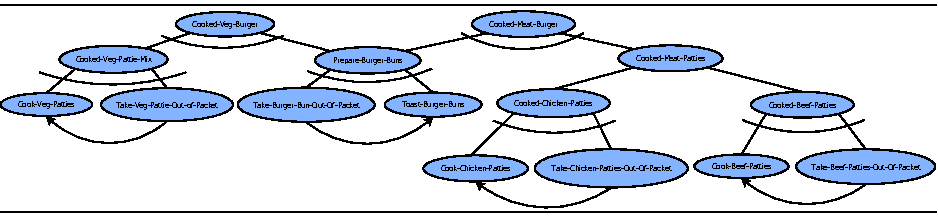
\includegraphics{images/example-plan-library.pdf}
}
\caption{Root-goals are nodes that have no parent nodes. Sub-goals are nodes that have both a parent and children and actions are nodes that have no children. And-nodes are represented by an undirected arc across the lines connecting the parent node to its children. Or-nodes do not have this arc. Actions or goals that are dependant on a previous action are represented by an arc with an arrow.}
\label{fig:example-plan-library}
\end{figure}

To elaborate on the above diagram one of A's top level or root-goals is \textit{Cooked-Veg-Burgers} it is an And-node and so means to accomplish it, requires successfully performing all of its children nodes. 

Children of Or-nodes such as \textit{Cooked-Meat-Patties} represent choices available to A to accomplish the root-goal. For example to achieve \textit{Cook-Meat-Patties} A could either accomplish \textit{Cooked-Chicken-Patties} or \textit{Cooked-Beef-Patties}.

Arrows represent dependencies between nodes. For example to be able to accomplish the action \textit{Cook-Beef-Patties}, A must first perform the action \textit{Take-Beef-Patties-Out-Of-Packet}.

Beginning the example, A first performs the action \textit{Take-Burger-Bun-Out-Of-Packet}, then proceeds to \textit{Toast-Burger-Buns}. At this point looking at the plan library we have two possible \textit{explanations} for A's behaviour, \textit{Cooked-Veg-Burger} or \textit{Cooked-Meat-Burger}.

Each of these explanations are equally likely at this point because the actions that have occurred so far could be part of either plan.

A then performs the action \textit{Take-Chicken-Patties-Out-Of-Packet}, given our assumptions we can conclude that A's root-goal is \textit{Cooked-Meat-Burger} and not \textit{Cooked-Veg-Burger}. In this way B has recognised A's plan thus performing the process of plan recognition.

\newpage

\section{Introduction to R.I.S.K.}

Developed and released by french film director Albert Lamorisse in 1957 as La Conqu\^ete du Monde, RISK is a turn-based board game for two to six players. This paper is only concerned with the standard version of R.I.S.K. which is an adversarial environment where players' vie to control a fully observable board portraying a static geographical map of the Earth.

\subsection{Equipment}

\begin{figure}[h]
\centering
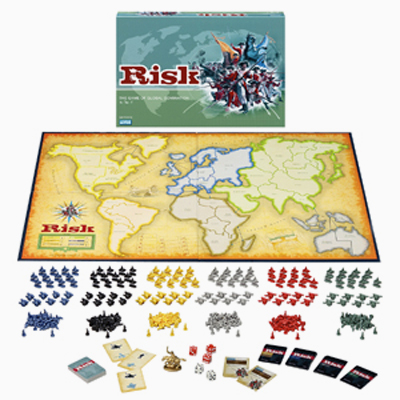
\includegraphics{images/risk-board}
\caption{Risk Equipment \cite{riskimage}}
\label{fig:risk-equipment}
\end{figure}

The game consists of three pieces of equipment:

\begin{itemize}
\item
A board portraying a geographical map of the earth.
\item
Different coloured tokens called \textit{armies}.
\item
Two sets of regular six-sided dice.
\item
A deck of forty-four cards.
\end{itemize}

\subsection{Rules}

The board is divided into forty two \textit{territories}. Each territory is a partition of the land mass of the Earth. These territories are further partitioned into six \textit{continents} usually corresponding to their real continent grouping.

Armies are placed in territories. If a player places an army in a territory, this declares that the player \textit{occupies} that territory. Players must have at least one army placed in a territory they own at all times. Players can choose to place as many additional armies as they wish in that territory.

How a player wins largely depends on the \textit{Game mode}. Game modes significantly impact the behaviour of players and is decided by players beforehand. In standard RISK they are:
\newline

\begin{tabular}{|l|p{11cm}|}
\hline 
\textbf{Game Mode} & \textbf{Description} \\ 
\hline 
Domination & Players aim to conquer a certain number of territories, \\ 
\hline 
Mission & Each player is given a single unique mission card. A mission card describes a state they must reach e.g. Occupy North America and Africa, for the rest of the game this is their \textit{root-goal} which only they know. In order to win they can either complete this root-goal or eliminate all other players. \\ 
\hline 
Capital Risk & Each player is given a Capital territory and to win a player must occupy all other Capital territories. \\ 
\hline
\end{tabular} 

This paper is concerned with the mission game mode \textbf{only}, therefore the following sections describe rules only for that game mode.

After an initial setup, each player's turn is split into three distinct phases which always occur in the same fixed order. These phases are:

\begin{enumerate}
\item
Reinforcement
\item
Attack
\item
Movement
\end{enumerate}

In each phase a player performs at least one discrete \textit{action} which helps to further the players goals, thus forming a sequential task environment.

\subsection{Turn Structure}

\subsubsection{Initial Setup}

The game begins with an initial setup, which involves:

\begin{itemize}
\item
Territories being equally divided in a random order between players.
\item
Players being given a number of starting armies. This number is calculated by taking an explicit number defined by the R.I.S.K rule book, which is inversely proportional to the number of players, and subtracting it from the number of territories the player owns. For example if there are three players, each player receives 35 starting armies and as there are 42 territories each player receives 14 territories. Therefore the number of remaining armies 35 subtract 14.
\item
Players distributing their starting armies over their territories.
\item
Each player being given a mission card.
\end{itemize}

\subsubsection{Reinforcement Phase}

At the start of a player's turn, they receive \textit{reinforcements} in the form of additional armies. The act of placing an army in a territory is called \textit{reinforcement}.  The number of additional armies received is based on the number of territories a player occupies and whether they occupy any continents.

\begin{table}[ht]
\centering
\begin{tabular}{|c|c|}
\hline 
\textbf{Occupied Continent} & \textbf{Number of Bonus Armies} \\ 
\hline 
Asia & 7 \\ 
\hline 
North America & 5 \\ 
\hline 
Europe & 5 \\ 
\hline 
Africa & 3 \\
\hline
Australia & 2 \\
\hline
\end{tabular}{}
\caption{Occupied Continent Army Reinforcement Bonus}
\label{table:continent-bonus}
\end{table}

\subsubsection{Attack Phase}

Once a player has distributed their armies from the reinforcement phase, they can choose to \textit{attack}. 

Territories occupied by a player that contain more than one army can attack neighbouring territories occupied by any other player. An attack consists of several \textit{battles}. The outcome of a battle is decided by means of rolling two sets of dice, thus making it a stochastic environment. One set is rolled for the \textit{defender} of the territory and the other for the \textit{attacker}. 

The number of dice each player receives for a battle is dependant on the number of armies placed in each of the players respective territories. The defender receives a die per army up to two armies. The attacker receives a die per army upto three armies not including the single army they are required to have in that territory while occupying it. 

The general rules of engagement are: dice rolls by each player are compared on a one-to-one basis in descending order of values. The player with the lower value at each comparison loses a single army though if the die are equal in value the attacker loses an army. The number of comparisons per battle are set by the number of dice the defending player has rolled. The attacking player can commence as many battles as they wish during an attack provided they have more than one army in the attacking territory.

An attack of a territory has three outcomes:

\begin{itemize}
\item
A \textit{FailedOccupation} by the attacker as they have only one army remaining in which case they must retreat and a \textit{SuccessfulDefence} by the defender who retains the territory.
\item
A \textit{FailedOccupation} by the attacker as they choose to retreat before having only one army remaining and a \textit{SuccessfulDefence} by the defender who retains the territory.
\item
A \textit{Successful-Occupation} by the attacker who occupies the territory and a \textit{FailedDefence} by the defender who has no armies remaining and so loses the territory. The attacking player, leaving at least one army behind, must then move armies from the territory they attacked from into the newly occupied territory.
\end{itemize}

A player can perform any number of attacks from any territory they own during their turn, provided they have more than one army in the territory they choose to attack from.

\subsubsection{Movement Phase}

When either the player chooses to end the attacking phase or can no longer attack because they do not occupy a territory which contains more than one army their movement phase begins.

During their movement phase a player may move armies from one territory to a neighbouring territory they own, provided they leave at least one army in the territory the armies were moved from. This action can only be done once per turn in this phase, after which the movement phase is finished.

After the movement phase has been completed the players turn ends and another players reinforcement phase begins.
\newpage

\subsection{Cards}

For each territory is a corresponding card. As well as name of that territory each card either depicts the symbol of an infantry, cavalry or artillery. By successfully occupying another player's territory in a turn, a player is then awarded a card and no more than one in that turn. Additionally there are two wild cards which can be substituted to represent a symbol of the players choosing. Owning a set of three cards with the same symbols or a set of three distinct symbols gives the player the opportunity to trade the set of cards for additional armies.

\section{Why Plan Recognition in Board Games}

NOT COMPLETE

By "knowing a users plan and goals can significantly improve the effectiveness of an interactive system" [Techniques for Plan Recognition]. Board games are most definately not exempt to this statement and With success seen in the application of plan recognition to video games, often in complex environments gives rise to ideas of transferring this sucess to board games.

Molineaux, Aha and Sukthankar believe that "plan recognition methods can be a powerful ally for machine learning techniques" \textbf{ref beating the defense}. Synnaeve and Bessiere also echo this belief with their work in StartCraft [\textbf{ref!}]. Their plan recognition agent utilized unsupervised machine learning to learn common plans which they then could fed this into an adaptive A.I. 

Since today, many program implementations of board games often contain an A.I. it is an attractive proposition to consider that by the same process of the Starcraft plan recognition agent. Plan recognition agents for board games could developed to augment board game A.I's with for example personalized plan librarys as Fagan and Cunningham suggest \textbf{[ref fagan and cunningham]} and by doing so build more interesting opponents for people to play against.

\section{Summary}

Plan recognition is an old area of research dating back to the 1950's. It has seen applications in a variety of fields including video games. R.I.S.K. a popular board game provides an interesting environment to test the application of plan recognition algorithms, having features such as being a multi-agent adversarial environment it intersects between classical board games which are often full observable deterministic environments, with elements of modern games such as stochiastic environments. Since plan recongition has been used before to augment A.I. for video games, there rises an opportunity to apply them to board games with techniques such as machine learning in-order to create more interesting A.I. opponents.

\chapter{Design}

\section{Introduction to PHATT}

WHY DID I CHOOSE PHATT?

PHATT was published by Christopher Geib and Robert Goldman in 2009 \cite{Geib:2009:PPR:1550966.1551246}. PHATT's approach is that plans are executed dynamically and the set of actions that an agent can take at each step, their \textit{pending set} depends critically on the actions that the agent has previously taken, this formed the basis of their model of plan execution.

The model is as follows. An agent would first choose a root-goal, then a set of plans to achieve that root-goal. Any actions of those plans that had no pre-requisite actions would form the initial pending set of the agent. The agent would then perform an action from the initial pending set and this would result in some actions being appended to the pending set and others being removed to form a new pending set. Assuming \textit{blind commitment} on the part of the agent, the agent would then continue to perform actions until it concluded the root goal had been achieved.

From this model, Geib and Goldman proposed an algorithm utilizing a Bayesian approach to perform probabilistic plan recognition. 

The algorithm computed \textit{Pr(g}|\textit{obs)}, the conditional probability of a root-goal \textit{g} given a set of observations \textit{obs} or its equivalent form \textit{Pr(exp}|\textit{obs)}, the conditional probability of a particular explanation \textit{exp} that the agent had a root-goal, given a set of observations \textit{obs}.

Using Bayes Rule they defined \textit{Pr(exp}|\textit{obs)} as:\newline

\centerline{
\textit{Pr(exp}|\textit{obs)} = \textit{Pr(exp} $\wedge$ \textit{obs)} / \textit{Pr(obs)}
}

They then (as other practical Bayesian systems do) exploited the equivalent formulae:\newline

\centerline{
\textit{Pr($exp_0$}|\textit{obs)} = \textit{Pr($exp_0$} $\wedge$ \textit{obs)} / $\displaystyle\sum\nolimits_{i}$ \textit{Pr($exp_i$} $\wedge$ \textit{obs)}
}

This is the conditional probability of the explanation $exp_0$ being computed by dividing the conditional probability of $exp_0$  by the sum of the probability mass associated with all possible explanations.

\subsection{Computing an Explanation's Probability}

To compute the term \textit{Pr(exp} $\wedge$ \textit{obs)} requires the plan library to be augmented with three probabilistic features:\newline

\begin{enumerate}
\item
The prior probability of the root-goal.
\item
The respective probabilities of choosing any sub-goals.
\item
The probabilities of picking actions from the agents pending set.
\end{enumerate}

The probability of an explanation is then calculated by multiplying each of the terms together in the following manner: \newline

\centerline{
\textit{Pr(exp} $\wedge$ \textit{obs)} = \textit{Pr}(\textit{goals})\textit{Pr}(\textit{plans}|\textit{goals})\textit{Pr}(\textit{obs}|\textit{exp})
}

\section{Environment Modelling and Design}

\subsection{Root-Goals}

The mission cards of the R.I.S.K. environment are the root-goals, these are:

\begin{itemize}
\item
Occupy Europe, Australia and one other continent.
\item
Occupy Europe, South America and one other continent.
\item
Occupy North America and Africa.
\item
Occupy North America and Australia.
\item
Occupy Asia and South America.
\item
Occupy Asia and Africa.
\item
Occupy 24 territories.
\item
Occupy 18 territories and occupy each with at least two troops.
\item
Eliminate a player.
\end{itemize}

As mission cards are handed out at random, the prior probability of a root-goal is 1/$n$ where $n$ is the number of mission cards. The data structure of a root-goal is therefore in the form of a tuple containing the name of the root-goal and its prior probability.

\centerline{
 $RG = ( rootGoalName, 1/n)$\newline
}

The collection of these data structures form the basis of the term \textit{Pr}(\textit{goals}) in the computation of \textit{Pr(exp} $\wedge$ \textit{obs)}.

A subset of these where the root-goal involved occupying continents only were chosen to be the focus of this paper. This choice was made due to time constraints and remains a definite avenue for future work. 

Root-goals involving occupying continents can be defined as one of two types:

\begin{enumerate}
\item
\textit{Two-Continent}: Players must occupy two explicitly named continents.
\item
\textit{Two-Continent+1}: Players must occupy two explicitly named continents and another of their choice.
\end{enumerate}

\textit{Two-Continent} are explicit in their sub-goals, but \textit{Two-Continent+1} type root-goals can be decomposed into \textit{children-root-goals}. Children-root-goals of a \textit{parent-root-goal} are a result of a different choice of sub-goals. The number of children-root-goals of a parent-root-goal depends on the environment. For example the root-goal Occupy Europe, South America and one other continent can be expressed as any of the following children-root-goals:

\begin{itemize}
\item
Occupy Europe, South America and Asia.
\item
Occupy Europe, South America and Africa.
\item
Occupy Europe, South America and North America.
\item
Occupy Europe, South America and Australia.\newline
\end{itemize}

Each is a valid root-goal in itself, but are still children of the same parent-root-goal. Therefore an assumption is made, where if the plan recognition agent predicts one of the children-root-goals when the players mission card is the parent-root-goal, it is classified as a correct prediction. A modelling difference followed this assumption.

By hard coding every root-goal as explanations of a players behaviour; then assigning that full set of explanations to each player from the start of the game, provided that action probabilities are computed, multiplied with each respective explanation, normalised and then stored immediately as soon as the action occurs. Removes the need to store a history of pending sets, to save a list of actions a player has taken or to create and calculate new instances of explanations. This method is similar to that of the 'Test and Generate' algorithm proposed in PHATTs paper rather than the dynamic algorithm proposed at the end of the paper.

Additonally this has another implicaton. Since PHATT computes \textit{Pr(exp} $\wedge$ \textit{obs)} by multiplying three terms together. Choosing to operate on a fully enumerated set of root-goals removes the need to compute player choice as we consider every case from the start hence the term \textit{Pr}(\textit{plans}|\textit{goals}) is equal to one for all explanations.

What is then measured over the course of the game is the probability of each explanation of a players behaviour, and the highest probability by the end of the game is the plan recognition agents prediction.

\subsection{Actions}

In R.I.S.K. the only actions players perform are:

\begin{itemize}
\item
Attacking Territories.
\item
Defending Territories.
\item
Occupying a Territory.
\item
Reinforcing Territories.
\item
Moving armies.
\item
Trading Territory Cards.
\end{itemize}

Each of these action must be modelled in a manner that contributes towards explanations of a player's behaviour.

\subsubsection{Attacking}

Though players can perform several attacks during their turn, they can only attack one territory at a time. Thus players' must choose both which territories to attack and the order in which to attack them, provided they have neighbouring territories and sufficient armies. Modelling these choices provides an avenue to infer a players plan.

The pending set of a player's attack actions for any turn is to either successfully or unsuccessfully attack territories they do not own, that are neighbour to atleast one territory that they own which also contains at least two armies.

If a player $p$ successfully occupies a territory $T_{o}$, then the attack actions of neighbouring territories of $T_{o}$ are added to $p$'s attack pending set. If they lose a territory $T_{l}$ due to another player's successful attack, then any attack actions of neighbouring territories of $T_{l}$ are removed from their attack pending set for their next turn. 

The attack action is a singular event that is either \textit{consistent} or \textit{inconsistent} with explanations of a players behaviour. 

For example given three explanations:

\begin{enumerate}
\item
Occupy North America and Australia.
\item
Occupy North America and Africa.
\item
Occupy Asia and South America.
\end{enumerate}

Successfully occupying a territory in North America would be \textit{consistent} with explanations 1 and 2, but \textit{inconsistent} with 3, or in probabilistic terms the likelihood of 1 and 2 would rise whereas 3 would fall.

Having defined the outcome of attacks as either successful or unsuccessful, attacks can be decomposed into following two actions: 

\begin{table}[ht]
\centering
\begin{tabular}{|c|c|p{8cm}|}
\hline 
\textbf{Action} & \textbf{Consistent}  & \textbf{Reasoning} \\ 
\hline 
Successful-Occupation & Yes & A good indication of a players plan is the territories they attack and successful attacks are in themselves the best outcome. \\ 
\hline 
FailedOccupation & Yes & Whether successful or not, attacking a territory is indicative of a players intention to occupy that territory and therefore a consistent action. Though a non-deterministic event, a FailedOccupation is in part due to a lack of armies which is suggestive that in cases the action has less significance than Successful-Occupation, as we could assume that players would choose not to attack if their chances of winning were poor.\\ 
\hline
\end{tabular}
\caption{Modelling Attack Actions}
\label{table:attack-modelling}
\end{table}

\newpage

\subsubsection{Defending}

Defending as opposed to attacking can be seen as a 'passive' action as an attack is required before a defence can occur. In that way the defence action is modelled as consistent or inconsistent with only the explanations it is directly related to. 

For example, given the three explanations from the previous section. If a \textit{SuccessfulDefence} were to occur in a territory in North America explanation one and two would be multiplied by a term $x$ which would be greater than 1, whereas explanation three would not be multiplied by anything. In the case of a \textit{FailedDefence} occurring in a territory in North America the same would occur but with $x$ in the range 0.9 < $x$ < 1.0. This model results in an interesting side-effect.

In PHATT at some point each explanations probability is normalised. The result is that explanations that were not multiplied by $x$ will inversely increase or decrease to explanations that were multiplied $x$. The more $x$ changes the value of an explanation the greater the difference will be in explanations that were not multiplied by $x$. To minimize this effect as big changes in explanation probabilities are undesirable for defence actions, the value of $x$ is kept in the range of 0.9 < $x$ < 1.1.

Defence in the same manner as attack can be either successful or unsuccessful, therefore defence can be decomposed into the following: 

\begin{table}[ht]
\centering
\begin{tabular}{|c|c|p{8cm}|}
\hline 
\textbf{Action} & \textbf{Consistent}  & \textbf{Reasoning} \\ 
\hline 
SuccessfulDefence & Yes & A successful defence of a territory may be purely a product of chance, but is more likely when they have a plan involving that territory. \\ 
\hline 
FailedDefence & No & An inconsistent action because a player would not normally allow a territory to be lost if it is a part of their plan. \\ 
\hline
\end{tabular}
\caption{Modelling Defence Actions}
\label{table:attack-defend-modelling}
\end{table}

\newpage

\subsubsection{Reinforce}

The reinforce actions that a player $p$ can perform at any turn $t$ is based solely on the territories that $p$ owns during turn $t$. The pending set of any players reinforce actions is therefore modelled as follows. 

For each territory $T$ that $p$ owns at a certain turn $t$. In $p$'s pending set is an action to reinforce $T$. If a territory $T_{l}$ is lost by $p$ (it is attacked then occupied by another player), its corresponding reinforce action is removed from the players pending set for the players turn at $t+1$. Conversely if another territory $T_{o}$ is occupied by $p$ then a reinforce action for $T_{o}$ is added to the players pending set at turn $t$.

\subsubsection{Movement}

The pending set of movement actions of player $p$ is the set of territories a player owns that are neighbour to a territory where $p$ has more than one army. Moving armies into a territory is modelled as a consistent action with the explanation that the territory that had armies moved into is directly related to.

\subsubsection{Trading Territory Cards}

Actions related to trading territory cards were not modelled. This is due to trading sets of cards only giving players bonus armies and the end effect of a player placing any number of armies is already captured by the current model.

\subsection{Territory}

Each territory is modelled as an entity. When a player occupies a territory the player gains access to a set of actions which together form that territories action set.

The action set of any territory is:

\begin{table}[ht]
\centering
\begin{tabular}{|c|c|}
\hline 
\textbf{Action} & \textbf{Description} \\ 
\hline 
Successful-Occupation & Attacking and occupying the territory.\\ 
\hline 
FailedOccupation & Attacking and failing to occupy the territory.\\ 
\hline 
SuccessfulDefence & Retaining the territory after an attack.\\ 
\hline 
FailedDefence & Losing the territory due to an attack.\\
\hline
Movement & Moving armies in to the territory.\\
\hline  
Reinforce & Placing armies in the territory.\\
\hline 
\end{tabular}
\caption{Territory Action Set}
\label{table:territory-actions-bonus}
\end{table}

\newpage

The data structure of a territory therefore is a triple containing the name of the territory the set of territory actions $TA$ and a set of references to the territories neighbours $TN$.

\centerline{
$T$ = $( territoryName, TN )$
}

A key concept in the design of the agent is that the pending set of a player is decided \textit{a priori} as it is based on the territories a player owns. By combining the action sets of each territory a player owns into a single set, all the actions a player can perform can be captured.

\subsection{Continent}

Each continent contains at least two territories and so can be modelled as a tuple of the name of the continent and the set of territories that are contained in that continent.

\centerline{
$C$ = $( continentName$, <$T_{1}$ ... $T_{n}$> $)$
}

\subsection{Player}

The term player has been and can be used inter changeably with the term agent. A defined data structure for a player is essential to be able to separate the numerous explanations of one player from another. The data structure must contain at least three features. A player name or ID, a list of territories they own $PT$ and a list of explanations $PE$.\newline

\centerline{
$P = ( playerName, PT, PE )$
}

\subsection{Explanations}

Explanations must be designed to contain all the necessary data required to compute its probability, it therefore contains these features:

\begin{itemize}
\item
The explanation name.
\item
A root-goal $RG$.
\item
A set of sub-goals $SGS$.
\item
A set of consistent actions $ECA$.
\item
A set of inconsistent actions $EIA$.
\end{itemize}

The resulting data structure is:\newline

\centerline{
$E = ( explanationName, RG, SGS, ECA, EIA )$
}

Inconsistent actions are stored in explanations due to modelling decisions as if it was the case that that if an action is not consistent then it is inconsistent then defence actions would be modelled incorrectly. Defence actions are not considered inconsistent to explanations that they are not directly related to, but would be if any actions not in the set of consistent actions are classified as inconsistent actions to an explanation.

Given the list of root-goals and sub-goals, the complete list of explanations is:

\begin{itemize}
\item
Occupy Europe, Australia and Africa.
\item
Occupy Europe, Australia and North America.
\item
Occupy Europe, Australia and South America.
\item
Occupy Europe, Australia and Asia.
\item
Occupy Europe, South America and Asia.
\item
Occupy Europe, South America and Africa.
\item
Occupy Europe, South America and North America.
\item
Occupy Europe, South America and Australia.
\item
Occupy North America and Africa.
\item
Occupy North America and Australia.
\item
Occupy Asia and South America.
\item
Occupy Asia and Africa.
\end{itemize}

\section{Prediction Agent Design}

\subsubsection{Building the Set of Explanations}

During the initialisation of the R.I.S.K. map, a set of explanations must be built for the environment to be later assigned to players. This first required the explicit specification of a root-goal and of sub-goals for each respective explanation in the environment, or in this context the Domination program. In addition it also required populating of each explanation with a set of consistent and inconsistent actions. This is done by the following operation:

\begin{pseudocode}[ruled]{generateExpList}{-}
\begin{algorithm}[H]
\ForAll {C $\in$ CS}{

	\ForAll {E $\in$ ES}{

		\If{C \textit{isSubGoalOf} E}{

			\ForAll{T $\in$ C}{

				\textit{addAction}(ReinforceT) to \textit{ECA}

				\textit{addAction}(MovementT) to \textit{ECA}
				\textit{addAction}(SuccessfulDefence) to \textit{ECA}
				\textit{addAction}{Successful-OccupationT} to \textit{ECA}
				\textit{addAction}(FailedOccupationT) to \textit{ECA} \newline

				\textit{addAction}(FailedDefenceT) to \textit{EIA}
			}
		}
	}
}
\end{algorithm}
\end{pseudocode}

The above pseudo code loops through the data structure of each continent $C$ in the set of continents $CS$. Each continent is checked against each explanation $E$ from the set of explanations' $ES$, for whether its name is contained in the set of sub-goals of each $E$ by the $isSubGoalOf$ operation. If true then the result is an if statement firing. 

The if statement contains a loop which iterates over the set territories in the loops current continent and using the $addAction$ operation, adds each territories action set to either the explanations consistent action $ECA$ or inconsistent action set $EIA$.

With a complete set of environment explanations $ES$, each player then allocated a unique instance of every explanation at the start of every game. 

\subsubsection{Computing Action Probabilities}

Since the sub-goal probabilities were removed and the root-goal prior probabilities are uniform, finding an appropriate method of computing \textit{Pr}(\textit{obs}|\textit{exp}), the probability of a player choosing an action from their pending set, was critical in the design of the plan recognition agent. 

To achieve this of course first presumes that we know what actions a player can perform and for that we require a method of generating a pending set of the available actions a player can perform. This is done by the following operation:

\begin{pseudocode}[ruled]{generatePS}{PT}
\begin{algorithm}[H]

$playerPS \gets $ $\emptyset$

\ForAll {T $\in$ PT}{

	\textit{addAction}(ReinforceT) to \textit{playerPS}

	\textit{addAction}(FailedDefenceT) to \textit{playerPS}

	\textit{addAction}(SuccessfulDefence) to \textit{playerPS}

	\ForAll{N $\in$ TN}{
			
		\eIf {playerOwnN}{

			\textit{addAction}(MovementT) to \textit{playerPS}
		}{

			\textit{addAction}(FailedOccupationT) to \textit{playerPS}
			\textit{addAction}(SucessfulOccupationT) to \textit{playerPS}
		}
	}

	\Return{playerPS}
}
\end{algorithm}
\end{pseudocode}

After initializing an empty pending set $playerPS$. The above pseudo code first loops through each territory $T$ in the list of all the territories that a player owns $PT$. For each territory a $ReinforceT$ action and a $LoseT$ action is added to $playerPS$. 

Before proceeding onto the next territory in $PT$ another loop is performed through the set of neighbouring territories $TN$ of that territory with an if-then-else statement. If the player owns that territory then the if condition $playerOwnN$ return true and a $MovementT$ action is added to $playerPS$, if not then a $OccupyT$ action is added to $playerPS$. After the operation the $playerPS$ is returned and can be cached if necessary.

With the $generatePS$ operation and an idea from a paper by Goldman, Geib and Miller \cite{Goldman99anew} which proposes weighting action probabilities towards consistent actions, a technique of doing so in the R.I.S.K. environment was required. Based on reasoning about the implications of an action to an explanation, consistent actions were positively weighted and inconsistent negatively weighted, but by how much is the crucial question?

The first approach to answer this was given a players pending set, the total number of actions are counted, these actions are then separated into consistent and inconsistent actions then a manually defined total weight is split among consistent and inconsistent respectively. For example out of a total action probability of 1.0, 0.5 would be distributed among consistent actions and 0.5 inconsistent actions. The idea behind this approach was that as the number of consistent actions decreased the likelihood of the them choosing the action given an explanation would in theory increase.

Unfortunately this approach proved to be problematic in cases where the number of consistent and inconsistent probabilities were significantly different and even detrimental in cases where the number of inconsistent actions were greater. 

For example, if there are:

\begin{itemize}
\item
2 Consistent actions and 4 Inconsistent actions, $Pr(cons)$ = 0.5 / 2 = 0.25 , $Pr(incons)$ = 0.5 / 4 = 0.125 
\item
4 Consistent actions and 2 Inconsistent actions. $Pr(cons)$ = 0.5 / 4 = 0.125, $Pr(incons)$ = 0.5 / 2 = 0.25
\end{itemize}

These significant differences in probabilities between actions resulted in large changes when multiplied by with the probability of an explanation, therefore it required an operation that would allow greater control over the weighting between consistent and inconsistent actions. The following pseudo-code details the operation:

\begin{pseudocode}[ruled]{computeBaseWeight}{w, pTotalActNum, pConsActNum}
\begin{algorithm}[H]

$sumWeight \gets w * consActNum$

$leftOver \gets 1.0 - sumWeight$

$base \gets leftOver / totalNumAct$

\Return{base}
\end{algorithm}
\end{pseudocode}

Given a predefined weight $w$, the total number of actions in a players pending set $pTotalActNum$ and the total number of consistent actions with an explanation $pConsActNum$. This operation computes a $base$ weight for all actions in a pending set by subtracting the total weight of the desired actions from 1, then distributing equally the remainder amongst all the actions in the players action set. This operation could easily be replaced with another such similar method.

Given the nature of the environment where the number of actions players can perform are relatively small, this method is suitable provided the weight difference is kept small. For environments where the number of consistent or inconsistent actions a player can perform are large, this may result in the value of $sumWeight$ becoming greater than one, making $leftOver$ negative, breaking the next calculation. Therefore a scalable method of controlling the weights between actions would be necessary in the design of such an agent for a larger action environment.

The operation $computeBaseWeight$ is part of a larger function which computes a $base$ value which the following $computeExpProb$ operation requires.

\begin{pseudocode}[ruled]{computeObsProb}{playerPS, totalExpConAct , obs}
\begin{algorithm}[H]
$expConAct \gets filterPS(totalExpConsAct, actType)$ \newline
$pTotalAct \gets filterPS(playerPS, actType)$\newline
$pTotalActNum \gets pTotalAct.size$ \newline

$pConsAct \gets $ $\emptyset$ \newline

\ForAll{A $\in$ \textit{pTotalAct}}{
			
	\If {A $\in$ \textit{expConsAct}}{

		\textit{addAction}(A) to \textit{pConsAct}
	}
}

$pConsActNum \gets pConsAct.size$\newline

$base \gets computeBaseWeight(w, pTotalActNum, pConsActNum)$\newline 

\Return $base$

\end{algorithm}
\end{pseudocode}

Given the players pending set $playerPS$ generated by the function $generatePS$, and the set of all consistent actions for an explanation $totalExpConAct$. Both the set of actions (must be of the type $obs$) a player can currently perform $pTotalAct$ and the consistent actions of the explanation can be be filtered using the $filterPS$ operation which given an action type and a set, removes all other action types from the given set. 

The set of $pTotalAct$ is then further filtered down into another set $pConsAct$ which contains only the consistent actions with the explanation. The sizes of $pConsAct$ and $pTotalAct$ are saved in two respective variables $pConsActNum$ and $pTotalActNum$.

Dividing these two variables effectively gives the proportion of available actions that a player can perform that are inconsistent and this fact is exploited by the next operation which is passed a predetermined weight and each variable to the $computeBaseWeight$ operation which returns the $base$ weight of an action. This base weight can easily be used to weight either inconsistent actions or consistent actions.

This formulae makes three assumptions:

\begin{enumerate}
\item
That any territories including ones that only contain one army can attack. Though this is not technically true, due to the nature of RISK where players are not restricted in any way on where they may place their armies during the reinforcement phase a player can practically attack any territory they do not own but have a territory they own neighbour to it at the start of their turn.
\item
That the likelihood of consistent attack actions are uniformly distributed.
\item
That the likelihood of inconsistent attack actions are uniformly distributed.
\end{enumerate}

\subsubsection{Computing Explanation Probabilities}

\begin{pseudocode}[ruled]{computeExpProb}{explanation, obs}
\begin{algorithm}[H]

\If{\textbf{not} alreadyIni}{ 

	$expProb \gets 1.0$

	$expProb \gets R * expProb$	
	
	$alreadyIni \gets true$
}

$playerPS \gets generatePS()$

$totalExpConsAct \gets ECA$

$weight \gets arbitraryNumber$ \newline

$base \gets computeObsProb(playerPS, totalExpConsAct, obs)$ 

$conActProb \gets base + weight$

$inConActProb \gets base$ \newline

\uIf{obs is consistent }{

	$expProb \gets conActProb * expProb$	

	
}\ElseIf{obs is inconsistent}{

		$expProb \gets inConActProb * expProb$

 }

$expProb \gets normalized(expProb)$

\Return{expProb}
\end{algorithm}
\end{pseudocode}

After initialising the float $expProb$, the term is multiplied by the root-goal prior $R$, this is done only when the explanation is first initialised and therefore the $alreadyIni$ flag is necessary. To complete the computation of an explanation, the operation $computeObsProb$ is applied to $obs$. Depending on whether $obs$ is consistent or not with the explanation, the appropriate action probability is multiplied with $expProb$ .

At this point in the operation $expProb$ is normalized, doing this is a deviation to the design of PHATT. Normalisation in PHATT of an explanations probability is normally only done when sampling of an explanation probability is required, not at the end of every operation. This design choice significantly decelerated the probability of any explanation from dropping to zero very quickly. As if an explanation probability did reach zero, its value would propagate over the data sample and so even if a consistent action were to occur that would normally raise the probability it would be multiplied by zero and so nothing would happen. 

\subsection{Example of Operation}

The concepts from this chapter can be tied together with an arbitrary example of computing \textit{Pr(exp}|\textit{obs)} the likihood of an explanation given an observation. The example will be extended to include the plan recongition agent handle two observations.


FIX PLAN LIBRARY CONNECTION FROM O-AS-SA TO AF MISTAKE

Assumptions for this example are:

\begin{itemize}
\item
Mission cards are unique between players and randomly handed out.
\item
Consistent attacks are assigned a weight $w$ of 0.02.
\item
When player $p_1$ attacks it is always a Successful-Occupation action.
\item
When player $p_1$ defends it is always a SuccessfulDefence action.
\item
The R.I.S.K map consists of only territories, continents and root-goals illustrated on Figure 3.1.
\end{itemize}

\begin{figure}[h]
\fbox{
	\centerline{
		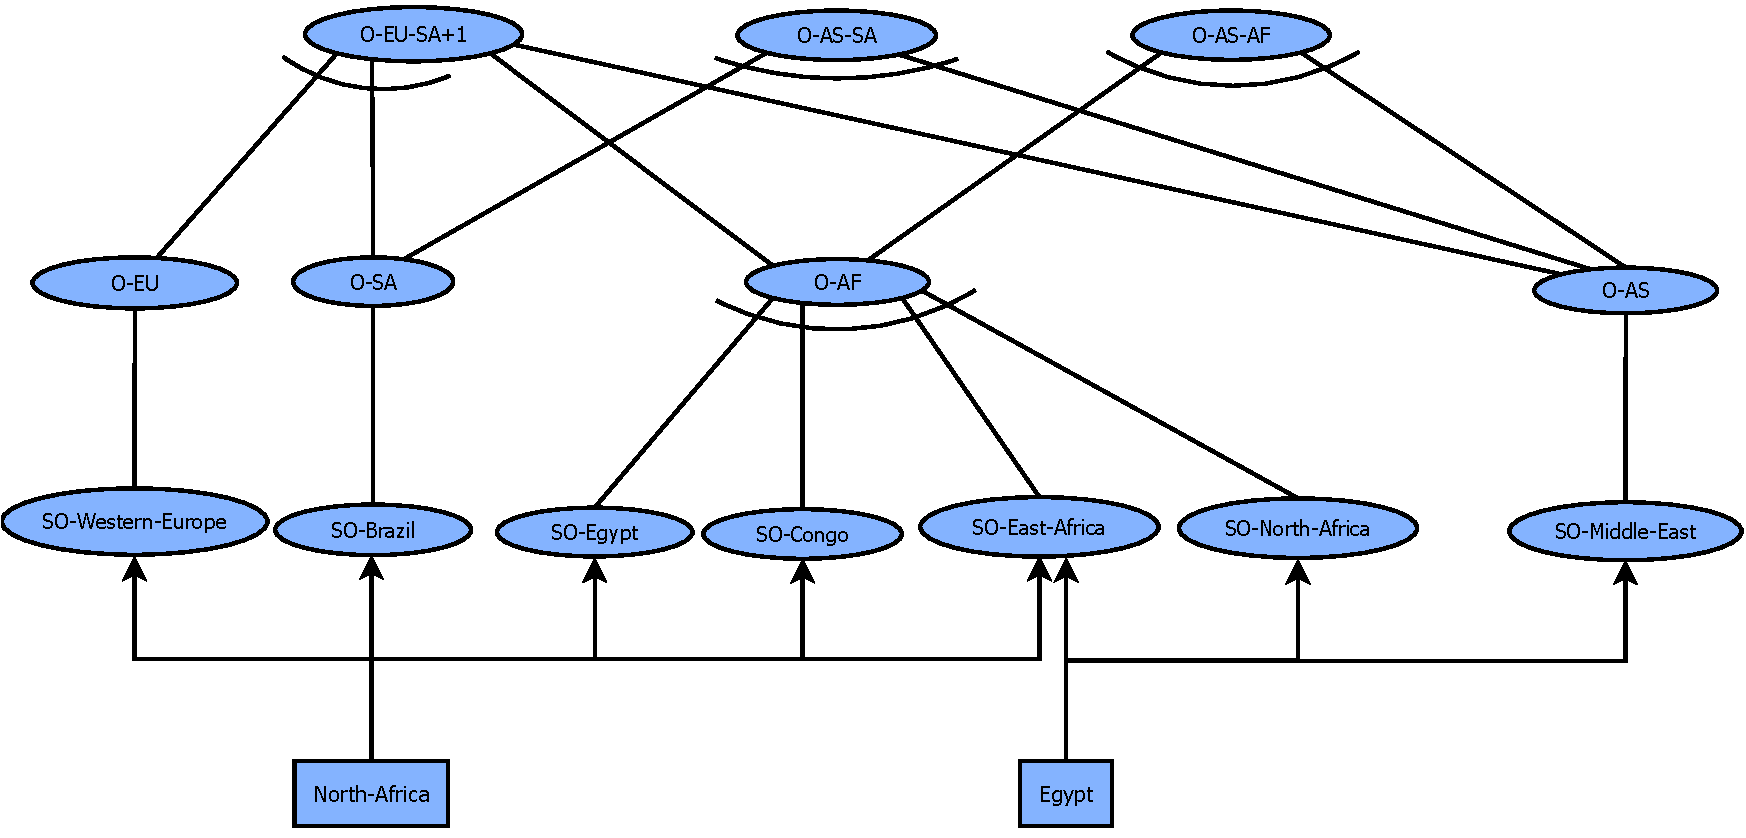
\includegraphics[width=\textwidth]{images/risk-plan-library.pdf}
	}
}
\caption{Successful-Occupation Plan Library for North-Africa \& Egypt}
\end{figure}

\newpage

The three root-goals of this environment are:

\begin{itemize}
\item
Occupy-Europe-South-America + One other continent (Occupy-EU-SA+1)
\item
Occupy-North-America-South-America (O-AS-SA)
\item
Occupy-South-America-Africa (O-SA-AF)
\end{itemize}

Each of the three root-goals have several sub-goals. In the context of mission R.I.S.K for a player to accomplish their root-goal they must have occupied every continent sub-goal, this is done through performing Successful-Occupation actions for every territory contained in that continent. 

Additionally squares represent territory entities. Arrows away from these squares are connected to the actions a player can perform by occupying this territory. This is done to represent the state of the world at the time the action was performed. For example by occupying the territory Egypt, it allows a player to perform the actions: O-East-Africa, O-North-Africa and O-Middle-East.

Recall the formulae:\newline

\centerline{
\textit{Pr(exp} $\wedge$ \textit{obs)} = \textit{Pr}(\textit{goals})\textit{Pr}(\textit{plans}|\textit{goals})\textit{Pr}(\textit{obs}|\textit{exp})
}

The term \textit{Pr}(\textit{goals}), the prior probability of each root-goal, is 1/\textit{n} where \textit{n} is the number of mission cards and therefore for this example is 1/3 for each explanation. 

The term \textit{Pr}(\textit{plans}|\textit{goals}) is 1.0 and so is not taken in account because the design of the plan recognition agent is to operate on on the full set of explanations, hence removing the need to calculate a choice.

The term \textit{Pr}(\textit{obs}|\textit{exp}) will be computed once an observation occurs in the example environment.

Player $p_1$ initially occupies the territory North-Africa and thus can perform actions connected to the North-Africa square. $p_1$ then performs a Successful-Occupation-Western-Europe action.

With an observation we can now compute the term \textit{Pr(exp} $\wedge$ \textit{obs)}, the probability of each explanation and O-Western-Europe for $p_1$.

First we must compute \textit{Pr}(\textit{obs}|\textit{exp}), the probability that $p_1$ would choose to perform the observation O-Western-Europe given each explanation.

\begin{itemize}
\item
Case 1 : \textit{Pr}(\textit{O-Western-Europe}|\textit{O-AS-AF})
\item
Case 2 : \textit{Pr}(\textit{O-Western-Europe}|\textit{O-EU-SA+1})
\item
Cast 3 : \textit{Pr}(\textit{O-Western-Europe}|\textit{O-AS-SA})
\end{itemize}

The plan recongition agent first applys the $computeExpProb$ operation to each of the above cases. Then using the $generatePS$ operation to build the full pending set for $p_1$.

After this the plan recognition agent retrieves a list of the all the consistent actions for each explanation by retrieving the $ECA$ set from each explanations data structure.

Given the observation O-Western-Europe, the complete pending set of the player, and the set $ECA$. The plan recognition agent uses the $computeObsProb$ operation to compute the probability of the Succesful-Occupation-Western-Europe.

For each explanation the $computeObsProb$ filters out all actions types except Successful-Occupation from both $p_1$ pending set and each $ECA$ set. The result is the Successful-Occupation actions that are consistent with the explanation $expConAct$ and a new pending set $pTotalActNum$ which contain the following Successful-Occupation actions:\newline

\centerline{
$p_1PS$ = \{O-Western-Europe, O-Brazil, O-Egypt, O-Congo, O-East-Africa\}
}

Given these two sets we both count the number of consistent actions that the players pending set contains for each respective explanation, by comparing what actions are contained in $pTotalActNum$ to each explanations $expConAct$ set and we count the total number of actions a player can perform $pTotalActNum$.

$pTotalActNum$ = 5

The counts given the action Successful-Occupation-Western-Europe is as follows:

\begin{table}[ht]
\centering
\begin{tabular}{|c|c|}
\hline 
\textbf{Explanation} & \textbf{Number of Consistent Actions} \\ 
\hline 
O-AS-AF & 0 \\ 
\hline 
O-EU-SA+1 & 1 \\ 
\hline 
O-AS-SA & 0 \\ 
\hline 
\end{tabular}
\caption{Consistent Action Count}
\label{table:territory-actions-bonus}
\end{table}

With these counts and our assumed $w$ the plan recognition agent can then compute a $base$ action probability for each explanation with the $computeBaseWeight$ operation as follows:

\begin{table}[ht]
\centering
\begin{tabular}{|c|c|c|c|}
\hline 
\textbf{Explanation} & TotalWeight & LeftOver & Base \ \\ 
\hline 
O-AS-AF & 0.02 * 0 & 1.0 - 0 & 0.2 \\ 
\hline 
O-EU-SA+1 & 0.2 * 1 & 1.0 - 0.02 & 0.196 \\ 
\hline 
O-AS-SA & 0.2 * 0 & 1.0 - 0 & 0.2 \\ 
\hline 
\end{tabular}
\caption{Consistent Action Count}
\label{table:territory-actions-bonus}
\end{table}

Consistent actions $cons$ are weighted so the probability of a consistent action $Pr(cons)$ = $base$ + $w$

Inconsistent actions $incons$ are not weighted so the probability of a inconsistent action $Pr(incons)$ = $base$

\begin{table}[ht]
\centering
\begin{tabular}{|c|c|c|}
\hline 
\textbf{Explanation} & $Pr(cons)$ & $Pr(incons)$ \ \\ 
\hline 
O-AS-AF & 0.2 & 0.2 \\ 
\hline 
O-EU-SA+1 & 0.216 & 0.196 \\ 
\hline 
O-AS-SA & 0.2 & 0.2 \\ 
\hline 
\end{tabular}
\caption{Consistent Action Count}
\label{table:territory-actions-bonus}
\end{table}

The plan recognition agent then computes \textit{Pr(exp} $\wedge$ \textit{obs)} by multiplying the term  \textit{Pr}(\textit{goals}) with one of the two action probabilities, depending on whether the action that was observed was consistent or not, in other words if was contained in $ECA$ or not.

For example to compute \textit{Pr(exp} $\wedge$ \textit{obs)} for the explanation O-EU-SA+1 the plan recongition agent would choose to multiply by $Pr(cons)$ and so the calculation would be 1/3 * 0.216. 

\begin{table}[ht]
\centering
\begin{tabular}{|c|c|}
\hline 
\textbf{Explanation} & \textit{Pr(exp} $\wedge$ \textit{obs)} \\ 
\hline 
O-AS-AF &  0.066 \\ 
\hline 
O-EU-SA+1 &  0.072 \\ 
\hline 
O-AS-SA & 0.066 \\ 
\hline 
\end{tabular}
\caption{Consistent Action Count}
\label{table:territory-actions-bonus}
\end{table}

\newpage

Finally to complete the calculation of \textit{Pr(exp}|\textit{obs)} the plan recognition agent normalises each with the following formula: \newline

\centerline{
\textit{Pr($exp_0$}|\textit{obs)} = \textit{Pr($exp_0$} $\wedge$ \textit{obs)} / $\displaystyle\sum\nolimits_{i}$ \textit{Pr($exp_i$} $\wedge$ \textit{obs)}
}

For example to compute \textit{Pr($exp$}|\textit{obs)} for O-EU-SA, the plan recognition agent would sum all explanation probablities which would work out as 

0.066 + 0.072 + 0.066 = 0.204 

Then it would divide the probability of O-EU-SA which is 0.072 by 0.204 which is 0.353.

\begin{table}[ht]
\centering
\begin{tabular}{|c|c|c|}
\hline 
\textbf{Explanation} &  \textit{Pr($exp$}|\textit{obs)} Pre-Normalisation &  \textit{Pr($exp$}|\textit{obs)} Post-Normalisation \\ 
\hline 
O-AS-AF & 0.066 & 0.324  \\ 
\hline 
O-EU-SA+1 &  0.072 & 0.353 \\ 
\hline 
O-AS-SA & 0.066 & 0.324 \\ 
\hline 
\end{tabular}
\caption{Consistent Action Count}
\label{table:territory-actions-bonus}
\end{table}

NEED TO ADD ANOTHER ACTION

Now another player $p_2$ attacks $p_1$.  $p_1$ then performs a SuccessfulDefence retaining the territory.

Incorporating these events is much simpler as probabilities are scaled down or up. Given the operations to compute the action probabilities for Successful-Occupation.

DEFEND ACTION - SuccessfulDefence action

REINFORCE ACTION - reinforce

\subsection{Conceptual Issues}

NOT COMPLETE

Main change is that PHATT works in an action space whereas I have had to adapt the implementation to represent the state of the 'risk world' for the algorithm to operate.

Using the constraints in the environment initially the model was based on the plan library proposed in the PHATT paper. This was not good therefore utilized the constraints of countries to narrow the number of possible explanations and actions.

Initially the movement model was based on the attack model where the smaller the number of actions the bigger the weighting should be, this is an incorrect model as the number of territories a player owns increases as a player gains more consistent movement and reinforce actions as they continue to be successful in their goal.

\section{Summary}

NOT COMPLETE

The summary for this section is

\chapter{Implementation}

Built purely in the Java programming language, the plan recognition agent follows the following \textit{event-driven} system architecture.

WHY DID I USE JAVA , WIDELY USE, COMPARATIVELY EASIER, WIDE RANGE OF LIBRARIES, GOOD IDES

\begin{figure}[h]
\centerline{
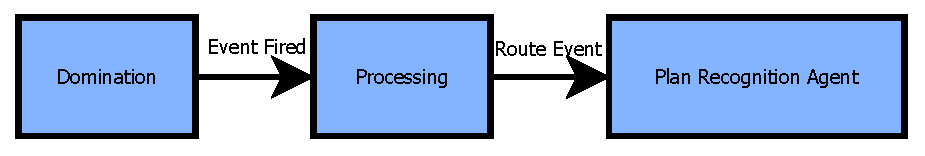
\includegraphics{images/event-driven-architecture}
}
\caption{Event-Driven Architecture}
\end{figure} 

To operate the plan recognition agent needs to be aware of several important aspects of the game. In particular: how many players there are, when the game begins, the games initial state, any changes that occur in the game and when the game is finished. These aspects can be broken down into individual events:

\begin{itemize}
\item
Start Game
\item
Player Initialisation
\item
Player Removal
\item
Territory Placement
\item
Successful Occupation
\item
Failed Occupation
\item
Army Movement
\item
Reinforcement
\item
End Game
\end{itemize}

When these occur a distinct event object is fired, these even objects contains important information about the event that is necessary to the plan recognition agent. These events are observed by the processing class which then routes them to the plan recognition agent. The plan recognition agent then looks at the received event object(s) and depending on the type of event object and the information held by it handles the object appropriately. The types of events, what they contain and their purpose are:

\begin{table}[ht]
\centerline{
\begin{tabular}{|c|p{6cm}|p{8cm}|}
\hline 
\textbf{Event Type} & \textbf{Contains Variables} & \textbf{Purpose} \\ 
\hline 
NewPlayer & playerName & Initialises a new player data structure with ID \textit{playerName}. \\ 
\hline 
RemovePlayer & playerName & Destroys the player data structure with ID \textit{playerName}. \\ 
\hline 
Successful-Occupation & attackerName, continentName, territoryName & Signals that the player named \textit{attackerName}  performed a Successful-Occupation. \\ 
\hline
FailedOccupation & attackerName, continentName, territoryName & Signals that \textit{attackerName} performed a FailedOccupation. \\ 
\hline
SuccessfulDefence & defenderName, continentName, territoryName & Signals that \textit{defenderName} performed a SuccesfulDefence. \\ 
\hline
FailedDefence & defenderName, continentName, territoryName & Signals that \textit{defenderName} performed a FailedDefence. \\ 
\hline
ArmyMovement & playerName, continentName, territoryName & Signals that \textit{playerName} performed an ArmyMovement. \\ 
\hline
Reinforce & playerName, continentName, territoryName & Signals that \textit{playerName} performed a Reinforce action. \\ 
\hline
\end{tabular}
}
\caption{Event Object Specification}
\label{table:event-description}
\end{table}

The architecture is such that the implementation of the plan recognition agent is not as dependant sub-component of the game, but rather a separate entity that operates in parallel to the game which if need be could be replaced by another plan recognition agent.

\section{Additional Implementation Concepts}

\subsection{Data Structure Re-Use}

The plan recognition agent makes use of the data structures from the game itself rather than the alternative of storing its own synchronized copy.

The advantages of this approach is less overhead as well significantly reducing the possibility that the plan recognition agents copy loses sync with the actual game state. 

On the other hand the disadvantage is that this makes the agent more dependant on the methods of the developers implementations.

\subsection{Google Guava Libraries}

The plan recognition agent makes extensive use of the freely available Google Guava libraries to allow the prediction agent to operate concurrently with the game as well as more efficiently in its operations.

\section{Summary}

The plan recognition agent was written in the Java programming language following an event-driven system architecture. It operated in parallel to the Domination program receiving events fired from the program to update data structures it held locally that contained information about each players explanation predictions.

\chapter{Evaluation} 

The evaluation plan consistend of three experiments with the plan recongition agent:

\begin{enumerate}
\item
Free Play
\item
Constrained Play
\item
A.I Play
\end{enumerate}

\textit{Free Play} can simply be described as human players "playing to win". In this manner it is how people would normally play mission R.I.S.K.

\textit{Constrained Play} consists of human players only performing actions that are directly-consistent with their root-goal.  More formally (excluding card related actions) given a set of actions, a player will only either:

\begin{itemize}
\item
Choose to attack a territory that is directly-consistent with their plan, or a territory that is on the shortest route to a territory that is directly consistent with their plan.
\item
Reinforce a territory that is directly-consistent with their plan, or a territory that is on the shortest route to a territory that is directly consistent with their plan.
\item
Moves armies to a territory that is directly-consistent with their plan, or a territory that is on the shortest route to a territory that is directly consistent with their plan.
\end{itemize}

This artificially constructed form of play is designed to be the easiest to perform plan recognition on due to the lack of environmental noise fron in-directly consistent and inconsistent actions found in other forms of play. In doing so a high correct prediction accuracy is expected and if this is not the case then the resulting experiments will provide a good indication into why.

\textit{A.I. Play} is games using the Domination programs existing implementations of A.I. players for its various game modes only. These A.I. players can be substituted for human players to the point where a game can consists of only A.I. players' fighting each other, and by doing so can complete a game in a fraction of the time that human players do. By automating the collection of these data samples using an free macro program called AutoHotkey \textbf{[ref to autohotkey]}, provided an opportunity for the collection of a large number of data samples to analyse. 

\section{Experimental Format}

There were two experiment formats, one for constrained play, the other for free play. Before any experiment the rules of the game were explained to participants. 

For constricted play, the particular play style required was described to participants.

For free play it was made clear to participants that there were two primary methods of winning in mission R.I.S.K. either by:

\begin{enumerate}
\item
Eliminating all other players from the game.
\item
Completing their mission card.
\end{enumerate}

At the end of the game participants were asked to give a short summary of their initial plan and any changes to that plan during the course of the game.

For the A.I. two experiments were performed with different values of $w$, 4 its normal setting and 100 a significantly higher value.

\newpage

\section{Data Collection}

After a game had finished the Domination program would generate a replay file, which if saved could be loaded at a later point through a specialised user interface for debugging created by the developers allowing a completely-independent and exact replay of the game.

\begin{figure}[h]
\centerline{
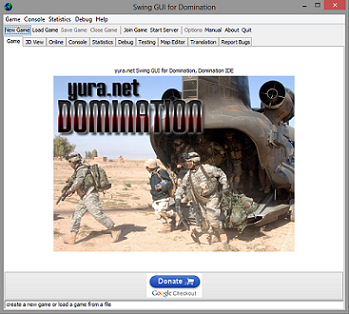
\includegraphics{images/domination-debug-gui.png}
}
\caption{Domination Debug Graphical User Interface}
\label{fig:dom-debug-gui}
\end{figure} 

Using this tool had significant implications, in that it would possible to re-observe games to assist with evaluation. It would also allow for testing of the plan recognition agent again with different modelling and/or calibrations in an exact same game and by doing so eliminate the environment as a variable between comparisons of the plan recognition agent.

In addition to Dominations replay file, the plan recognition agent would simultaneously generate a csv file recording the significant features of a game, namely:

\begin{itemize}
\item
Which player won and which players' lost.
\item
Each players actual mission.
\item
The probabilities of each players explanations over the course of the game.
\end{itemize}

Scripts written in the Python programming language were then used to automate the analysis of these generated csv files.

\newpage

\section{Experimental Findings}

Experiments with the plan recognition agent revealed the following insights:

\begin{enumerate}
\item
The accuracy of the prediction agent is 32.61\% better than random guess.
\item
The prediction accuracy of the plan recognition agent is highest in constrained play. 
\item
The prediction accuracy of the plan recognition agent is HOW MUCH PERCENT higher for players who won than players who lost.
\item
The prediction accuracy of the plan recognition agent is significantly higher for human players than the domination A.I. players.
\item
From the prediction accuracy of the plan recognition agent, we can infer when the domination A.I. gives less significance to completing its missions.
\item
The length of game has a positive effect on the accuracy of the prediction agent.
\end{enumerate}

Keeping in mind the initial hypothesis, we attempt to evaluate whether plan recognition algorithms are beneficial in games, specifically R.I.S.K.

To do this we first comment on general trends, then we explore two questions for both human and A.I players:

FIX THIS SECTION, TALK ABOUT WHAT YOU DEFINE AS IN GENERALC

CLARIFY STRUCTURE MORE

The following sections will be made up of evaluating prediction accuracy in general, for winners and losers, asking two essential questions throught out.

\begin{itemize}
\item
Does the plan recognition agent converge on the correct explanation?
\item
How fast does the plan recongition agent converge on the correct explanation?
\end{itemize}

\subsection{Explanation Convergence Format}

PICTURE OF STANDARD SUCCESSFUL CONVERGENCE OF AN EXPLANATION

At the start of a game forty-two turns are required to place one army on each territory of the R.I.S.K map. These observations are not taken into account as the distribution of territories between players is automatic and random. 

After this the remaining initial armies are distributed by players on to their territories. During this the probability of explanations that are consistent with the actions a player is performing will slowly rise and conversely those that explanations which with the actions are inconsistent will slowly fall.

Once this initial setup is complete (which could be from 80 to 120 turns depending on the number of players) the attack phase begin for the first player $p_c$, at this time the probabilities of $p_c$ explanations may change rapidly depending on the number of actions that $p_c$ performs in their turn. The most significant change occurs when there is a high number of actions. This is due to the plan recognition agents model which has been built to give attack actions the greatest significance.

After $p_c$ turn is over, other players begin their attack phases in-turn, and unless the action another player performs is to attack a territory owned by $p_c$, the probabilities of $p_c$ explanations remained unaffected. 

This continues till the end of the game at which point the probability of a players explanation will have either converged successfully or unsuccessfully to the correct explanation. 

\subsection{Prediction Accuracy in General}

Given there are six mission cards, the accuracy of a random guess of a players mission card is 16.67\%. According to Table 7.1, at its worse the plan recognition agent in general performs 8.47\% better than this, and at its best 63.72\% better. 

Of free and constrained play table 7.1 reveals that \textit{constrained play had a significantly higher accuracy than both free and A.I. play}. This is unsurprising given its artificial nature. Designed to be ideal the scenario for the plan recognition agent, it is therefore in itself not a good measure of evaluating the success of the plan recognition agent, but in conjunction with Free Play gives us a better picture of how well the plan recognition agent performed.

We then ask why and why not, did it converge.

\begin{figure}[h]
\centerline{
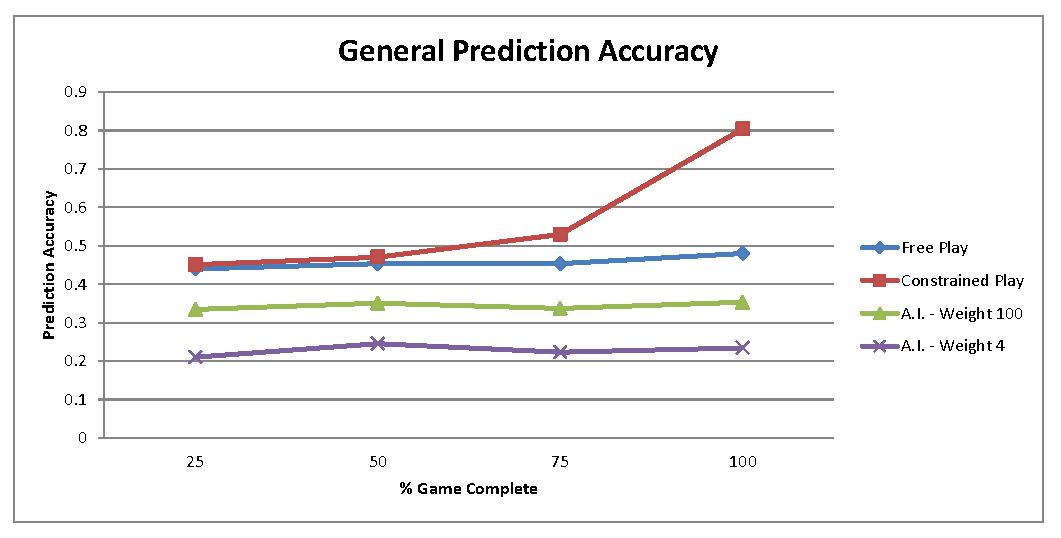
\includegraphics[width=\textwidth]{images/general-graph.pdf}
}
\caption{General Prediction Accuracy}
\label{fig:dom-debug-gui}
\end{figure} 

Figure 5.2 details the general prediction accuracy of the plan recongition agent at intervals of 25\% of the games duration. From this we can infer several important trends.

In general the plan recongition of the different types of play the plan recongition agent performed significantly better in \textit{constrained play had a than both free and A.I. play}. This is unsurprising given its artificial nature. Designed to be ideal the scenario for the plan recognition agent, it is therefore in itself not a good measure of evaluating the success of the plan recognition agent, but in conjunction with Free Play gives us a better picture of how well the plan recognition agent performed.

In general the plan recongition agent performed better on human players than A.I. players. The reason for this is due primarily to the way in which the humans and the A.I. differ in operation. According to the A.I developer at Yura.Net "the mission A.I. is a minimal extension of the core play. Since the core logic is reasonably good at conquering continents and eliminating opponents it just has it's decisions skewed a little to make sure it's going after the right continent/player without causing it to generally play poorly. "

Changing the variable $w$ hence explains the plan recognition agents increase in accuracy of up to \%10  as the A.I.'s deciesions becomes more skewed towards occupying mission continents and less towards occupying accessible non mission-continents and eliminating opponents both of which are observed as inconsistent actions by the plan recognition agent.

There is a significant increase in the predicition accuracy of the plan recognition agent in constrained play in the 75 to 100\% of game play complete range. This is because in the later part of any game players can perform more actions per turn due to the increasing number of armies on the board.

Why in general does the 



An analyis of the plan recognition agents accuracy in general is not sufficient, as it ignores that there are in fact two distinct types of player of R.I.S.K. which are:

\begin{enumerate}
\item
\textit{Winners} - a player who have successfully occupied their mission continents
\item
\textit{Losers} - players who have failed to do so.
\end{enumerate}

\subsection{Winner-Loser Prediction Accuracy}

How the game is played out for each player or their \textit{game-scenarios}, deciedes whether a player is a winner or loser.  The main game-scenarios that the plan recognition agent faces are the following:

Winners who won \textit{quickly} or \textit{slowly} and who spent the majority of their game:

\begin{itemize}
\item
fighting over non-mission continents.
\item
fighting over mission continents.
\end{itemize}

Losers who were eliminated \textit{quickly} or \textit{slowly} or who were \textit{not-eliminated} and who spent the majority of their game:

\begin{itemize}
\item
fighting over non-mission continents.
\item
fighting over mission continents.
\end{itemize}

These cases can be compactly represented in a definitional framework.

\begin{table}
\centerline{
\begin{tabular}{cc|c|c|c}
\cline{3-4}
&  & Mission & Non-Mission \\ 
\cline{1-4}
\multicolumn{1}{  |c| }{\multirow{2}{*}{Winner} } &
\multicolumn{1}{  c| }{Quickly} & & & \\ \cline{2-4}
\multicolumn{1}{ |c  }{}                        &
\multicolumn{1}{ |c| }{Slowly} & & & \\ \cline{1-4}
\multicolumn{1}{ |c  }{\multirow{3}{*}{Loser} } &
\multicolumn{1}{ |c| }{Quickly} & & & \\ \cline{2-4}
\multicolumn{1}{ |c  }{}                        &
\multicolumn{1}{ |c| }{Slowly} & & & \\ \cline{2-4}
\multicolumn{1}{ |c  }{} 						&
\multicolumn{1}{ |c| }{Not-Eliminated} & & & \\ \cline{1-4}					
\end{tabular}
}
\caption{Game-Scenario Table}
\label{table:ga,e-scenariol-table}
\end{table}

Using table 5.1 we classify players into their game-scenarios on game-by-game basis. As there can be only one winner, the winner row only ever has one entry, whereas the loser row can have 1 to 5 entries.

By definition in cases where a player performs action on non-mission continents \textit{only}, the plan recognition agent cannot produce a correct prediction. By establishing this extreme, if we view the degree of fighting over mission and non-mission continents as a scale, the higher the proportion of actions on mission continents to non-mission continents, the higher the likelihood of the prediction agent is likely to be correct. NEED TO PROVE CLAIM?

\subsubsection{Prediction Accuracy of Winners}

\begin{figure}[h]
\centerline{
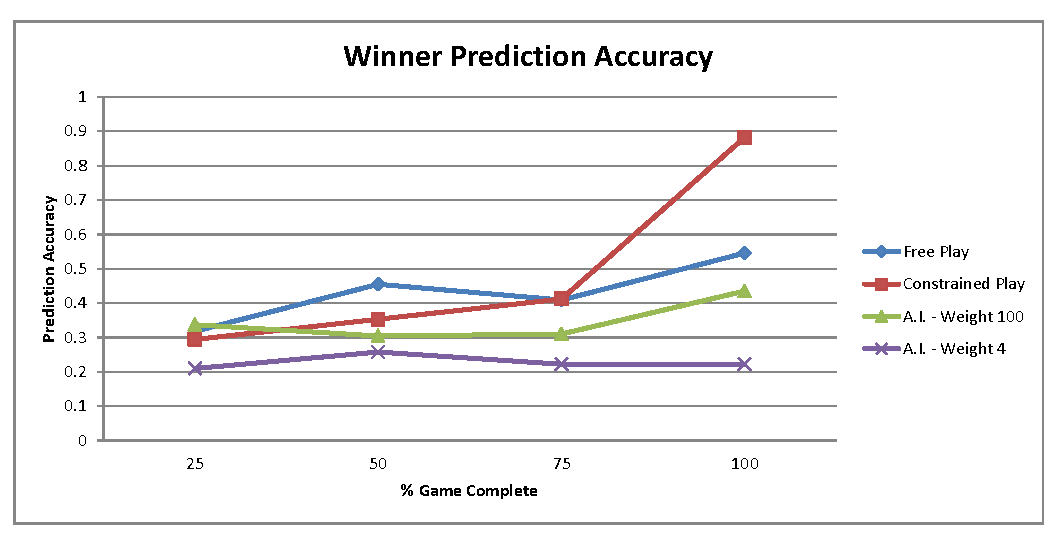
\includegraphics[width=\textwidth]{images/winner-graph.pdf}
}
\caption{Winner Prediction Accuracy}
\label{fig:dom-debug-gui}
\end{figure} 

Comparison of the Figure 5.3 to figure 5.4 shows that in every type of play the plan recognition agents \textit{prediction accuracy of winners is better than that of losers}. The plan recognition agent is more successful at predicting due to a number of reasons:

Winners by definition have successfully performed their mission or will have eliminated every player, in either case they will have performed each consistent action for a mission atleast once. Making on average as the data reflects the number of consistent actions performed by the winner, on average higher than that of losers hence making it easier to detect.

On the other hand though there are ofcourse cases where the plan recognition agent is unsucessful: 

There are cases where a winners has occupied the entire last continent for their mission in one turn and since sampling is done on a turn by turn basis the plan recognition agent will miss the significant change in probabilities as the system does not register an end of turn but rather a different event which is the end of the game.

Therefore the shorter the game the more likely the prediction will be correct for the winner. GET DATA TO SUPPORT THIS! 

\subsubsection{Prediction Accuracy of Losers}

\begin{figure}[h]
\centerline{
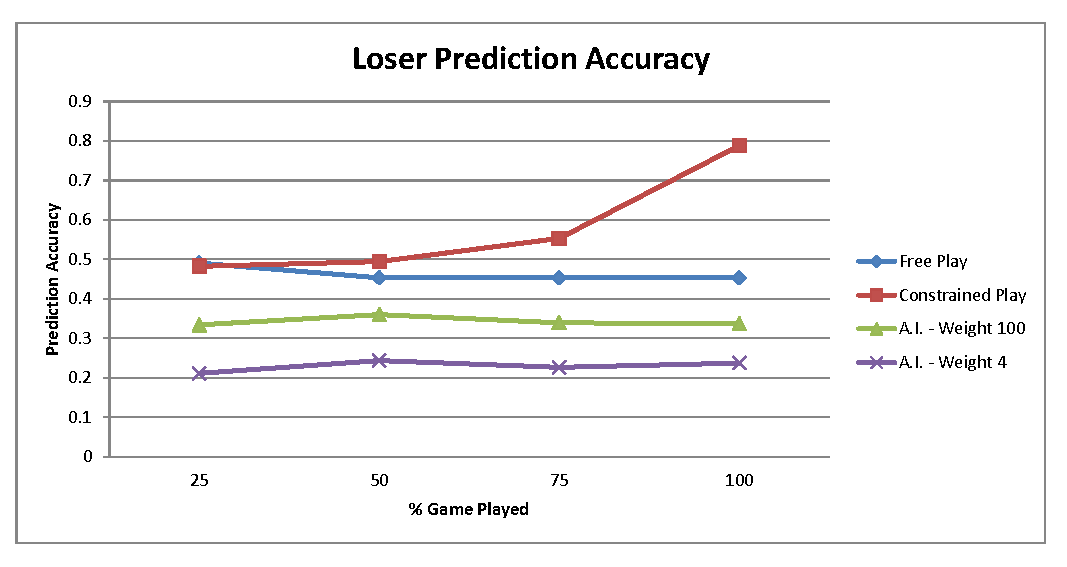
\includegraphics[width=\textwidth]{images/loser-graph.pdf}
}
\caption{Domination Debug Graphical User Interface}
\label{fig:dom-debug-gui}
\end{figure} 

GENERAL REASONS WHY LOSER ACCURACY IS WORSE

Losers who were eliminated early

Losers are often prevented from successfully achieving their goal.

Present typically examples where this is the case.

Winners who win quickly

Winners who win slowly

Though there were exceptions to this? Misclassification due to association?

We will describe each case, present a hypothesis for the plan recognition agents prediction accuracy then present examples from the data for most significant of these cases to support the hypothesis. 

Why is the accuracy of winners better than losers? May be because weighting of attack actions is towards successful attacks, of which winners perform more.

but this is not necessarily true winners just like losers may be in positions where they cannot perform actions that are directly-consistent.

A proportion of incorrect predictions occur because losers can be eliminated resulting in a lack of data about the losers behaviour. If a loser was to be eliminated early on in the game then their explanations probabilities would \textit{flat-line}, in that the prediction does not change for the remainder of the game. If the loser had been performing more inconsistent actions then consistent actions up until that point then the prediction will be wrong, inversely it may be correct for the very same reason.

WINNERS CONSTRAINED PLAY

Table 7.4 shows two incorrect predictions for winners in constrained play. Both were \textit{Two-Continent+1} mission types and from analysis of each both are shown to be incorrect for the same reason. 

SHOW A GRAPH OF ONE EXAMPLE OF WINNER CONSTRAINED WRONG

The final prediction probabilities of the above graph was split exactly equally between two different children-root-goals as their sub-goals were identical, thus resulting in an incorrect or argueably \textit{inconclusive} prediction.

It will not converge clearly in the case a player performs only actions that are consistent with more than one explanation.

\subsubsection{Explanation Accuracy}

In what way does overlap of missions between players effect predictions? Is it negative or positive, or is it both?

Do certain explanations perform better? Why?

Constrained play two-continents appear to be better.

Definite trend that two-continent-missions are predicted worse than others for a.i, very poor accuracy for weight 4.
 
Do the accuracy of missions with two continents appear on average to be better? No

For A.I. Play, winner and loser - Why is it that Europe-South-America-One is better than the rest when trend is normally two-continent accuracy is better? Explore this

The number of data samples are quite small.	Why is it that there are no winners for the missions Asia-South-America and Asia-Africa. Is this because these mission cards are harder?

Would make sense seeing as there is a trend in other data showing lower percentage accuracy for that mission.

Accuracy of two-continent missions appear in general to be better.

Asia-Africa appear to be lower prediction accuracy on average the A.I. play type, Asia is the hardest continent to occupy and therefore this might be causing the prediction accuracy to be the lowest, as players may not often choose to take Asia first first even if it is in their mission.

Is the prediction accuracy of any mission with Asia in it worse? Could get a good indication of frequency of losers to winners with missions involving Asia. Do a total across all plays of number of winners and losers.

In the context of constrained play, players do not purposely seek to hinder the progress of other players' missions. The winner of constrained play is often the player with the least overlapping mission with other players and the smallest number of territories to occupy. This situation allows for a player to quickly complete their mission with little opposition from other players who do not interfere.

SHOW THAT CONSTRAINED PLAY GAMES ARE ON AVERAGE SHORTER THAN OTHER GAME TYPES CAN DO WITH GRAPH

\subsection{Prediction Analysis for A.I. Players}

AI 100 LOSERS GETS WORSE OVER GAME LENGTH

BIG DROP IN PREDICTION ACCURACY IN A.I 4 GAME OVERS 210 IN TURNS BUT SINCE THE NUMBER OF SAMPLES MUST BE SMALL HAS A LOW EFFECT ON THE GENERAL ACCURACY

Since the A.I. for the game has its decisions skewed, varying this should in theory cause the A.I. to perform either better or worse depending on whether decisions are skewed towards decisions that are more consistent with the mission or away from decisions that are consistent with the mission but are rather focused on occupying continents that the A.I. has advantages in or eliminating players who are weak.

The variable that decides this to what degree decisions are skewed we will refer to as $w$.

Two experiments were performed with different values of $w$, 4 its normal setting and 100 a significantly higher value.

The prediction accuracies were in tables ....

Now we could make the argument that, 

Look at the length of the game, if length of the game is generally longer for weight 4 than weight 100, then we can propose that on weight 4

Each A.I. is better and therefore game is longer
Each A.I is worse and therefore game is longer

There is a significant improvements in the prediction accuracy of the plan recognition agent from $w$4 to $w$100 and if the aim of the A.I. was to perform its mission quickly and in doing so effectively then this would be confirmed by the readings from the plan recognition agent.

\section{Summary}

\chapter{Conclusion}

\subsection{Nature of Game}

The nature of R.I.S.K. is adversarial and in-order to achieve ones own mission, players either directly or indirectly eliminate each other and must modify their own plan in order to survive or prevent other players from winning. 

Given the model these changes in behaviour are see as directly-inconsistent with their own mission and rather seems consistent with whatever explanation that those actions \textit{are} directly consistent with instead.

Given this environment and the high-level of overlap between missions the results are misclassification.

For example:

PRESENT EXAMPLE

\subsection{Simplicity of Model}

Players who spend a game fighting over a single continent raise the probability of all explanations associated with that continent and the result is a prediction of several explanations being equally likely. This also applies to fighting over two continents that are part of a three continent explanation.

Inherent issues with PHATT as is unable to deal with deception[ref] and often players must perform actions unrelated to a plan to be able to complete their plan e.g survive, have to conquer other non-relevant continents, this confuses the algorithm.

Misclassification's occur due to three(keep looking in data) main reasons:

by Association - Explanations appear likely because players do things related to them even though they haven't done anything in one of the continents e.g Europe SA, Asia appears likely even though there has been occupation of territories in Europe because of lots of activity in SA and Asia. This issue is slightly negated by how I have modelled the attack actions probability contribution to explanations

\subsection{Improvement of Model}

HOW TO FIX

Solving this problem could be done in potentially two ways either:

Identifying actions are in-directly consistent and modelling them to accurately contribute to explanations - further modelling to further diffferentiate noise from meaninggul behaviour.
 
Giving greater weights to actions that are directly consistent through the state of the game  more significant - making noise less significant.

For example, knowing that a player owns four out of five of a continents territories when they choose to attack the last territory is intuitively more significant to the explanation of the player wanting to own that continent then if they only owned a single continent of that territory and choose to attack another territory.

Use a system of tiered consistent actions!

ExplanationProb = ExplanationProb * Weight

The weight for each consistent action is flat at the moment or more precisely actions are consistent in themselves but may not be consistent given the \textit{context} of the game state. To deal with this, we should introduce into our calculations data from the game state.

For example

Making a system of applying weights in a manner that is proportional to the state of the game e.g

Weight = 0.1 * 1- (The proportion of consistent actions for that explanations) * (Proportion of territories a player owns of the continents) <- Proportion of reinforce actions available to the player.

Best case = Low Number of consistent actions and high number of territories owned e.g

Has 1 attack option out of 13 and owns 9 of the ten territories

0.1 * 1-(1/13) * 9/10 

Worst Case = High number of consistent actions and low number of territories owned

0.1 * 1-(12/13) * 4/10 

Has 12 attack options out of 13 and owns 4 of the ten territories

What is the weight was computed in the normal manner but would be scaled up down by two factors in-order to make an action that appear
Plans should consider not only consider what occurs in the action space but the state of the environment as well.

\section{Main insights and results}

The main insights and results from this...

Free and A.I. play are definitely a more natural form of playing. Players in these perform actions that are either indirectly-consistent or inconsistent primarily because their plan at that point may be different to that of their mission. So a better measure for the general accuracy of the plan recognition  agent for humans is rather Ftree Play as prediction accuracies of human players is most significant. Therefore \textit{the plan recognition agent is 32.61\% better than random guess} and so we can establish that the plan recognition agent indeed does converge on the correct explanation 49.28\% of the time.

\section{Outcomes}

Players don't ignore their mission card like at first predicted, as long as the mission appears easier to complete than eliminating all other players, then players will try achieve their mission.

In evaluation DO NOT JUST RELY ON MEASUREMENTS! DISCUSS OUTCOMES! MAKE INFERENCES FROM DATA!

THE WHOLE PURPOSE OF ACADEMIA IS TO LEARN, SHOW THAT YOU HAVE SOMETHING TO CONTRIBUTE TO THAT AIM TO LEARN!

What did you do that you found easy? What did you do that you found hard? 

Would you recommend doing something, what would you recommend not doing?

TALK ABOUT THE OUTCOMES OF YOUR WORK!

\section{Criticism}

Essentially attack has been modelled following PHATT but the rest of the actions are simple given a weighting of 0.98 for inconsistent and 1.0 for consistent. Thus attack has been modelled as the most significant action in the environment and this we can intuitively tell is not the case.

MODEL IS LOP SIDED TOWARDS ATTACK, SHOULD TAKE INTO ACCOUNT WHAT TERRITORIES PLAYERS OWN AT THE END OF A TURN.

ATTACK probability COMPUTATIONS, TREATS ANY NON OWNED CONNECTED TERRITORY AS ATTACKABLE, GOES ON ASSUMPTION THAT PLAYER HAS AT LEAST TWO ARMIES IN EVERY TERRITORY

Small number of data samples for free play and constrained winners, therefore analysis will likely not have covered all the cases.

Calculation problems, give example of a explanation with more territories being higher than one with fewer even though the fewer one was correct.

How to differentiate between two identical alternates? E.g prediction is equal between EU SA AU and EU AU SA 

Sampling of probability needs to be more frequent rather than just at end of term as many actions occur between turns and the game may end in the middle of a lot of actions during one turn. Players do a lot of significant things in one turn.

\section{Future Work}

A.I. play was done with six players, would be interesting to see the effects on prediction accuracy on games with different number of players.

THINK ABOUT WHY IT WOULD IMPROVE

\subsection{Model Augmentation}

\subsubsection{Application of Machine Learning}

Allow for method choice probabilities again and use machine learning to computer better sub-goal choice probabilities based on preferences shown in training data.

\subsubsection{More Sophisticated Action Probability Computations}

The application of more sophisticated computation models based on the idea of generating a pending set from the state of the world then performing calculations with that pending set.

Probability model changed to PROPORTION SYSTEM of consistent actions * 0.1 
0.9 - proportion for consistent probability
1 - proportion for inconsistent probability

\subsubsection{More Sophisticated Modelling of Current Model}

Players in these perform actions that are either indirectly-consistent or inconsistent  primarily because their plan at that point may be different to that of their mission. Either type of action reduces the probability of the correct explanation given the current model. MODEL TO TAKE THIS INTO ACCOUNT

The model can be augmented further as any action could in fact be further decomposed into two types,\textit{directly-consistent} or \textit{indirectly-inconsistent}. For example a directly-consistent action would be to occupy a territory of an explanation, where as an indirectly-consistent action would be a player breaking another players continent by occupying a territory in that continent, as preventing other players from completing their mission makes completing ones own mission more likely. This distinction has not been taken into account as any action that is not directly-consistent is classified as an inconsistent action in the model and investigation into the effects of doing some may yield improvements.

Only attack actions have been modelled in a manner other than scaling up by 1.02 and down by 0.98 to simulate the effects of small decreases and increases in likelihood. More sophisticated computation models of action probabilities could be investigated to capture the state of the game to a greater degree in each calculation rather than scaling.

Other than modelling attacks as two events where the result affect both involved players, the model does not considered the effects. This could be improved by

Model does not take into account situations where players cannot perform any consistent actions and therefore any action that a player performs is considered inconsistent but actually could be indirectly-consistent. This could be improved by

The model does not take into account the importance of territories. Each continent has a number of territories which control entry into the continent. To elaborate each continent has a fixed number of these entry territories and if it were possible for a player to perfectly defend only the entry territories and occupy the remaining territories of the continent they would in theory never lose the continent as players must occupy the entry territory to be able to occupy other territories in that continent. The model does not take into consideration this.

Look at where player has already placed armies and figure out a probability based on where they place armies. Argument though is placement is not restricted an form.

\subsubsection{Extension to Include Other Types of Mission Cards}

Extension of the model to include other mission cards. Due to the design, eliminating players could be modelled but modelling Occupy 24, 18 due to design decision has such high overlap with all other missions it would be hard to model this.

A proposed method of modelling eliminating player missions

Eliminating player mission cards - some system where data of who is being consistently attacked is recorded and probabilities are multiplied by a number based on number of attack actions for a player and number of territories that player has remaining.

\subsection{Discussion of Possible Applications}

Using the plan recognition software given a programs a plan to detect how well a program performs a plan. 

Using genetic algorithms to perform meta optimisation this is done by randomly assigning a choice weight to the ai then looking at the numbers returned by the plan recognition algorithm and choosing the best configuration that survived and won.

\section{Summary of whole report}

A platform has been setup for further improvements of the model.

Why because they are an artificially derived benefit which can be used by a player to optimize their behaviour, not solely , but in conjunction with the results of a plan recognition system.

WHY USE THIS ALGORITHM WHY IS SUITABLE END ON A POSITIVE NOTE

\chapter{Appendix}

\section{Accuracy Count Measurements}

\subsection{General Prediction Accuracy}

\begin{table}[ht]
\centerline{
\begin{tabular}{cc|c|c|c|c|c|c|c|c|}
\cline{3-10}
& & \multicolumn{8}{ c| }{\textbf{\% Game Played}} \\
\cline{3-10}
& & \multicolumn{2}{ c| }{25} & \multicolumn{2}{ c| }{50} & \multicolumn{2}{ c| }{75} & \multicolumn{2}{ c| }{100} \\ \cline{3-10} 
\hline 
\multicolumn{1}{ |c| }{\textbf{Type of Play} }& \textbf{Player Type} & \textbf{C} & \textbf{I} & \textbf{C} & \textbf{I} & \textbf{C} & \textbf{I} & \textbf{C} & \textbf{I} \\ 
\hline 
\multicolumn{1}{ |c| }{\multirow{2}{*}{Free} } & Winner & 7  & 15  & 10 & 12 & 9 & 13 & 12 & 10 \\ 
\cline{2-10}
\multicolumn{1}{ |c| }{} & Loser & 26 & 27 & 24 & 29 & 25 & 28 & 24 & 29 \\ 
\hline 
\multicolumn{1}{ |c| }{\multirow{2}{*}{Constrained} } & Winner & 5 & 12 & 6 & 11 & 7 & 10 & 15 & 2 \\ 
\cline{2-10}
\multicolumn{1}{ |c| }{} & Loser & 41 & 44 & 42 & 43 & 47 & 38 & 67 & 18 \\ 
\hline
\multicolumn{1}{ |c| }{\multirow{2}{*}{A.I. - Weight 100} } & Winner & 62 & 122 & 56 & 128 & 57 & 127 & 80 & 104 \\ 
\cline{2-10}
\multicolumn{1}{ |c| }{} & Loser & 307 & 613 & 331 & 589 & 312 & 608 & 310 & 610 \\  
\hline
\multicolumn{1}{ |c| }{\multirow{2}{*}{A.I. - Weight 4} }  & Winner & 35 & 132 & 43 & 124 & 37 & 130 & 37 & 130 \\ 
\cline{2-10}
\multicolumn{1}{ |c| }{} & Loser & 176 & 659 & 203 & 632 & 189 & 646 & 198 & 637 \\ 
\hline
\end{tabular}
}
\caption{Winner-Loser Game-Length Correct-Incorrect Prediction Count, \textbf{C} = Correct, \textbf{I} = Incorrect}
\label{table:winner-loser-accuracy}
\end{table}

\begin{table}[ht]
\centerline{
\begin{tabular}{c|c|c|c|c|c|c|c|c|}
\cline{2-9}
& \multicolumn{8}{ c| }{\textbf{\% Game Played}} \\
\cline{2-9}
& \multicolumn{2}{ c| }{25} & \multicolumn{2}{ c| }{50} & \multicolumn{2}{ c| }{75} & \multicolumn{2}{ c| }{100} \\ \cline{3-9} 
\hline 
\multicolumn{1}{ |c| }{\textbf{Type of Play} }& \textbf{C} & \textbf{I} & \textbf{C} & \textbf{I} & \textbf{C} & \textbf{I} & \textbf{C} & \textbf{I} \\ 
\hline 
\multicolumn{1}{ |c| }{\multirow{1}{*}{Free} } & 33 & 42 & 34 & 41 & 34 &41 & 36 & 39 \\ 
\cline{2-9}
\hline 
\multicolumn{1}{ |c| }{\multirow{1}{*}{Constrained} } & 46 & 56 & 48 & 54 & 54 & 48 & 82 & 20\\ 
\cline{2-9}
\hline
\multicolumn{1}{ |c| }{\multirow{1}{*}{A.I. - Weight 100} } & 369 & 735 & 387 & 717 & 372 & 732 & 390 & 714 \\ 
\cline{2-9}
\hline
\multicolumn{1}{ |c| }{\multirow{1}{*}{A.I. - Weight 4} } & 211 & 791 & 246 & 756 & 224 & 778 & 235 & 767 \\  
\cline{2-9}
\hline
\end{tabular}
}
\caption{General Game-Length Correct-Incorrect Prediction Count, \textbf{C} = Correct, \textbf{I} = Incorrect}
\label{table:winner-loser-accuracy}
\end{table}

\newpage

\subsection{Free Play}

\begin{table}[ht]
\centerline{
\begin{tabular}{|c|c|c|c|}
\hline 
\textbf{Mission} & \textbf{Correct} & \textbf{Incorrect} & \textbf{\% Accuracy} \\ 
\hline 
Occupy-Europe-Australia-One & 6 & 9 & 40.00 \\  
\hline 
Occupy-Asia-South-America & 8 & 4 & 66.67 \\ 
\hline
Occupy-Europe-South-America-One & 8 & 11 & 42.11 \\
\hline
Occupy-North-America-Africa & 5 & 6 & 45.45 \\
\hline
Occupy-Asia-Africa & 5 & 5 & 50.00 \\
\hline
Occupy-North-America-Australia & 4 & 4 & 50.00 \\
\hline
\end{tabular}
}
\caption{Free Play General Accuracy}
\label{table:free-general-accuracy}
\end{table}

\begin{table}[ht]
\centerline{
\begin{tabular}{|c|c|c|c|}
\hline 
\textbf{Mission} & \textbf{Correct} & \textbf{Incorrect} & \textbf{\% Accuracy} \\ 
\hline 
Occupy-Europe-Australia-One & 3 & 2 & 60.00 \\  
\hline 
Occupy-Asia-South-America & 2 & 1 & 66.67 \\ 
\hline
Occupy-Europe-South-America-One & 0& 3 & 0.00 \\
\hline
Occupy-North-America-Africa & 4 & 1 & 80.00 \\
\hline
Occupy-Asia-Africa & 1 & 1 & 50.00 \\
\hline
Occupy-North-America-Australia & 2 & 2 & 50.00 \\
\hline
\end{tabular}
}
\caption{Free Play Winner Accuracy}
\label{table:free-winner-accuracy}
\end{table}
		
\begin{table}[ht]
\centerline{
\begin{tabular}{|c|c|c|c|}
\hline 
\textbf{Mission} & \textbf{Correct} & \textbf{Incorrect} & \textbf{\% Accuracy} \\ 
\hline 
Occupy-Europe-Australia-One & 3 & 7 & 30.00 \\  
\hline 
Occupy-Asia-South-America & 6 & 3 & 66.67 \\ 
\hline
Occupy-Europe-South-America-One & 8 & 8 & 50.00 \\
\hline
Occupy-North-America-Africa & 1 & 5 & 16.67 \\
\hline
Occupy-Asia-Africa & 4 & 4 & 42.86 \\
\hline
Occupy-North-America-Australia & 2 & 2 & 50.00 \\
\hline
\end{tabular}
}
\caption{Free Play Loser Accuracy}
\label{table:free-loser-accuracy}
\end{table}	

\newpage

\subsection{Constrained Play}

\begin{table}[ht]
\centerline{
\begin{tabular}{|c|c|c|c|}
\hline 
\textbf{Mission} & \textbf{Correct} & \textbf{Incorrect} & \textbf{\% Accuracy} \\ 
\hline 
Occupy-Europe-Australia-One & 13 & 4 & 76.47 \\  
\hline 
Occupy-Asia-South-America & 16 & 1 & 94.12 \\ 
\hline
Occupy-Europe-South-America-One & 10 & 7 & 58.82 \\
\hline
Occupy-North-America-Africa & 12 & 5 & 70.59 \\
\hline
Occupy-Asia-Africa & 15 & 2 & 88.24 \\
\hline
Occupy-North-America-Australia & 16 & 1 & 94.12 \\
\hline
\end{tabular}
}
\caption{Constrained Play General Accuracy}
\label{table:constrained-general-accuracy}
\end{table}

\begin{table}[ht]
\centerline{
\begin{tabular}{|c|c|c|c|}
\hline 
\textbf{Mission} & \textbf{Correct} & \textbf{Incorrect} & \textbf{\% Accuracy} \\ 
\hline 
Occupy-Europe-Australia-One & 1 & 1 & 50.00 \\  
\hline 
Occupy-Asia-South-America & 0 & 0 & 0.00 \\ 
\hline
Occupy-Europe-South-America-One & 4 & 1 & 80.00 \\
\hline
Occupy-North-America-Africa & 5 & 0 & 100.00 \\
\hline
Occupy-Asia-Africa & 0 & 0 & 0.00 \\
\hline
Occupy-North-America-Australia & 5 & 0 & 100.00 \\
\hline
\end{tabular}
}
\caption{Constrained Play Winner Accuracy}
\label{table:cons-winner-accuracy}
\end{table}
		
\begin{table}[ht]
\centerline{
\begin{tabular}{|c|c|c|c|}
\hline 
\textbf{Mission} & \textbf{Correct} & \textbf{Incorrect} & \textbf{\% Accuracy} \\ 
\hline 
Occupy-Europe-Australia-One & 12 & 3 & 80.00 \\  
\hline 
Occupy-Asia-South-America & 16 & 1 & 94.12 \\ 
\hline
Occupy-Europe-South-America-One & 6 & 6 & 50.00 \\
\hline
Occupy-North-America-Africa & 7 & 5 & 58.33 \\
\hline
Occupy-Asia-Africa & 15 & 2 & 88.24 \\
\hline
Occupy-North-America-Australia & 11 & 1 & 91.67 \\
\hline
\end{tabular}
}
\caption{Constrained Play Loser Accuracy}
\label{table:constrained-loser-accuracy}
\end{table}	

\newpage

\subsection{A.I. Play - Weight 100}

\begin{table}[ht]
\centerline{
\begin{tabular}{|c|c|c|c|}
\hline 
\textbf{Mission} & \textbf{Correct} & \textbf{Incorrect} & \textbf{\% Accuracy} \\ 
\hline 
Occupy-Europe-Australia-One & 51 & 133 & 27.72 \\  
\hline 
Occupy-Asia-South-America & 50 & 134 & 27.17 \\ 
\hline
Occupy-Europe-South-America-One & 127 & 57 & 69.02 \\
\hline
Occupy-North-America-Africa & 58 & 126 & 31.52 \\
\hline
Occupy-Asia-Africa & 37 & 147 & 20.11 \\
\hline
Occupy-North-America-Australia & 67 & 117 & 36.41 \\
\hline
\end{tabular}
}
\caption{A.I. Play General Accuracy - Weight 100}
\label{table:ai-100-general-accuracy}
\end{table}

\begin{table}[ht]
\centerline{
\begin{tabular}{|c|c|c|c|}
\hline 
\textbf{Mission} & \textbf{Correct} & \textbf{Incorrect} & \textbf{\% Accuracy} \\ 
\hline 
Occupy-Europe-Australia-One & 15 & 21 & 41.67 \\  
\hline 
Occupy-Asia-South-America & 9 & 9 & 50.00 \\ 
\hline
Occupy-Europe-South-America-One & 9 & 8 & 52.94 \\
\hline
Occupy-North-America-Africa & 15 & 21 & 41.67 \\
\hline
Occupy-Asia-Africa & 14 & 28 & 33.33 \\
\hline
Occupy-North-America-Australia & 18 & 17 & 51.43 \\
\hline
\end{tabular}
}
\caption{A.I. Play Winner Accuracy - Weight 100}
\label{table:ai-100-winner-accuracy}
\end{table}
			
\begin{table}[ht]
\centerline{
\begin{tabular}{|c|c|c|c|}
\hline 
\textbf{Mission} & \textbf{Correct} & \textbf{Incorrect} & \textbf{\% Accuracy} \\ 
\hline 
Occupy-Europe-Australia-One & 36 & 112 & 24.32 \\  
\hline 
Occupy-Asia-South-America & 41 & 125 & 24.70 \\ 
\hline
Occupy-Europe-South-America-One & 118 & 49 & 70.66 \\
\hline
Occupy-North-America-Africa & 43 & 105 & 29.05 \\
\hline
Occupy-Asia-Africa & 23 & 119 & 16.20 \\
\hline
Occupy-North-America-Australia & 49 & 100 & 32.89 \\
\hline
\end{tabular}
}
\caption{A.I. Play Loser Accuracy - Weight 100}
\label{table:ai-100-loser-accuracy}
\end{table}			

\newpage

\subsection{A.I. Play - Weight 4}

\begin{table}[ht]
\centerline{
\begin{tabular}{|c|c|c|c|}
\hline 
\textbf{Mission} & \textbf{Correct} & \textbf{Incorrect} & \textbf{\% Accuracy} \\ 
\hline 
Occupy-Europe-Australia-One & 34 & 133 & 20.36 \\  
\hline 
Occupy-Asia-South-America & 27 & 140 & 16.17 \\ 
\hline
Occupy-Europe-South-America-One & 88 & 79 & 52.69 \\
\hline
Occupy-North-America-Africa & 28 & 139 & 16.77 \\
\hline
Occupy-Asia-Africa & 9 & 158 & 5.39 \\
\hline
Occupy-North-America-Australia & 49 & 118 & 29.34 \\
\hline
\end{tabular}
}
\caption{AI Play General Explanation Accuracy - Weight 4}
\label{table:ai-4-general-accuracy}
\end{table}

\begin{table}[ht]
\centerline{
\begin{tabular}{|c|c|c|c|}
\hline 
\textbf{Mission} & \textbf{Correct} & \textbf{Incorrect} & \textbf{\% Accuracy} \\ 
\hline 
Occupy-Europe-Australia-One & 6 & 27 & 18.18 \\  
\hline 
Occupy-Asia-South-America & 8 & 21 & 27.59 \\ 
\hline
Occupy-Europe-South-America-One & 14 & 20 & 41.18 \\
\hline
Occupy-North-America-Africa & 3 & 13 & 18.75 \\
\hline
Occupy-Asia-Africa & 1 & 28 & 3.45 \\
\hline
Occupy-North-America-Australia & 5 & 21 & 19.23 \\
\hline
\end{tabular}
}
\caption{AI Play Winner Explanation Accuracy - Weight 4}
\label{table:ai-4-winner-accuracy}
\end{table}

\begin{table}[ht]
\centerline{
\begin{tabular}{|c|c|c|c|}
\hline 
\textbf{Mission} & \textbf{Correct} & \textbf{Incorrect} & \textbf{\% Accuracy} \\ 
\hline 
Occupy-Europe-Australia-One & 28 & 106 & 20.90 \\  
\hline 
Occupy-Asia-South-America & 19 & 119 & 13.77 \\ 
\hline
Occupy-Europe-South-America-One & 74 & 59 & 55.64 \\
\hline
Occupy-North-America-Africa & 25 & 126 & 16.56 \\
\hline
Occupy-Asia-Africa & 8 & 130 & 5.80 \\
\hline
Occupy-North-America-Australia & 44 & 97 & 31.21 \\
\hline
\end{tabular}
}
\caption{AI Play Winner Explanation Accuracy - Weight 4}
\label{table:ai-4-loser-accuracy}
\end{table}

\section{Game Length Correct-Incorrect Prediction Count}

\begin{table}[ht]
\centerline{
\begin{tabular}{cc|c|c|c|c|c|c|c|c|c|c|}
\cline{3-12}
& & \multicolumn{10}{ c| }{\textbf{Number of Game Turns}} \\
\cline{3-12}
& & \multicolumn{2}{ c| }{< 120} & \multicolumn{2}{ c| }{ 120-150} & \multicolumn{2}{ c| }{ 150-180} & \multicolumn{2}{ c| }{ 180-210} & \multicolumn{2}{ c| }{ 210+} \\ \cline{3-10} 
\hline 
\multicolumn{1}{ |c| }{\textbf{Type of Play} }& \textbf{Player Type} & \textbf{C} & \textbf{I} & \textbf{C} & \textbf{I} & \textbf{C} & \textbf{I} & \textbf{C} & \textbf{I} & \textbf{C} & \textbf{I}\\ 
\hline 
\multicolumn{1}{ |c| }{\multirow{2}{*}{Free} } & Winner & 11 & 10 & 1 & 0 & 0 & 0 & 0 & 0 & 0 & 0 \\ 
\cline{2-12}
\multicolumn{1}{ |c| }{} & Loser & 22 & 28 & 2 & 1 & 0 & 0 & 0 & 0 & 0 & 0 \\ 
\hline 
\multicolumn{1}{ |c| }{\multirow{2}{*}{Constrained} } & Winner & 15 & 2 & 0 & 0 & 0 & 0 & 0 & 0 & 0 & 0 \\ 
\cline{2-12}
\multicolumn{1}{ |c| }{} & Loser & 67 & 18 & 0 & 0 & 0 & 0 & 0 & 0 & 0 & 0 \\ 
\hline
\multicolumn{1}{ |c| }{\multirow{2}{*}{A.I. - Weight 100} } & Winner & 9 & 12 & 20 & 35 & 20 & 22 & 17 & 23 & 14 & 12 \\ 
\cline{2-12}
\multicolumn{1}{ |c| }{} & Loser & 36 & 69 & 100 & 175 & 65 & 145 & 71 & 129 & 38 & 92 \\  
\hline
\multicolumn{1}{ |c| }{\multirow{2}{*}{A.I. - Weight 4} } & Winner & 3 & 7 & 7 & 31 & 13 & 34 & 12 & 26 & 2 & 32 \\ 
\cline{2-12}
\multicolumn{1}{ |c| }{} & Loser & 11 & 39 & 50 & 140 & 59 & 176 & 41 & 149 & 37 & 133 \\ 
\hline
\end{tabular}
}
\caption{Game-Length Correct-Incorrect Prediction Count, \textbf{C} = Correct, \textbf{I} = Incorrect}
\label{table:winner-loser-accuracy}
\end{table}

\begin{table}[ht]
\centerline{
\begin{tabular}{c|c|c|c|c|c|c|c|c|c|c|}
\cline{2-11}
& \multicolumn{10}{ c| }{\textbf{Number of Game Turns}} \\
\cline{2-11}
& \multicolumn{2}{ c| }{< 120} & \multicolumn{2}{ c| }{120-150} & \multicolumn{2}{ c| }{150-180} & \multicolumn{2}{ c| }{180-210} & \multicolumn{2}{ c| }{210+} \\ \cline{3-11} 
\hline 
\multicolumn{1}{ |c| }{\textbf{Type of Play} }& \textbf{C} & \textbf{I} & \textbf{C} & \textbf{I} & \textbf{C} & \textbf{I} & \textbf{C} & \textbf{I} & \textbf{C} & \textbf{I} \\ 
\hline 
\multicolumn{1}{ |c| }{\multirow{1}{*}{Free} } & 33 & 38 & 3 & 1 & 0 & 0 & 0 & 0 & 0 & 0 \\ 
\cline{2-9}
\hline 
\multicolumn{1}{ |c| }{\multirow{1}{*}{Constrained} } & 82 & 20 & 0 & 0 & 0 & 0 & 0 & 0 & 0 & 0 \\ 
\cline{2-9}
\hline
\multicolumn{1}{ |c| }{\multirow{1}{*}{A.I. - Weight 100} } & 45 & 81 & 120 & 210 & 85 & 167 & 88 & 162 & 52 & 108 \\ 
\cline{2-9}
\hline
\multicolumn{1}{ |c| }{\multirow{1}{*}{A.I. - Weight 4} } & 14 & 46 & 57 & 171 & 72 & 210 & 53 & 175 & 39 & 163 \\  
\cline{2-9}
\hline
\end{tabular}
}
\caption{General Game-Length Correct-Incorrect Prediction Count, \textbf{C} = Correct, \textbf{I} = Incorrect}
\label{table:winner-loser-accuracy}
\end{table}

\newpage

\section{Graphs}

\begin{table}
\centerline{
\begin{tabular}{cc|c|c|c}
\cline{3-4}
&  & Mission & Non-Mission \\ 
\cline{1-4}
\multicolumn{1}{  |c| }{\multirow{2}{*}{Winner} } &
\multicolumn{1}{  c| }{Quick} & & & \\ \cline{2-4}
\multicolumn{1}{ |c  }{}                        &
\multicolumn{1}{ |c| }{Slow} & & & \\ \cline{2-4}
\multicolumn{1}{ |c  }{\multirow{3}{*}{Loser} } &
\multicolumn{1}{ |c| }{Quick} & & & \\ \cline{1-4}
\multicolumn{1}{ |c  }{}                        &
\multicolumn{1}{ |c| }{Slow} & & & \\ \cline{2-4}
\multicolumn{1}{ |c  }{} 						&
\multicolumn{1}{ |c| }{Till End} & & & \\ \cline{1-4}							
\end{tabular}
}
\end{table}

\begin{table}[ht]
\centerline{
\begin{tabular}{cc|c|c|c|c|c|c|c|c|c|c|}
\cline{3-12}
& & \multicolumn{10}{ c| }{\textbf{Turns}} \\
\cline{3-12}
& & \multicolumn{2}{ c| }{< 120} & \multicolumn{2}{ c| }{ 120-150} & \multicolumn{2}{ c| }{ 150-180} & \multicolumn{2}{ c| }{ 180-210} & \multicolumn{2}{ c| }{ 210+} \\ \cline{3-10} 
\hline 
\multicolumn{1}{ |c| }{\textbf{Type of Play} }& \textbf{Player Type} & \textbf{C} & \textbf{I} & \textbf{C} & \textbf{I} & \textbf{C} & \textbf{I} & \textbf{C} & \textbf{I} & \textbf{C} & \textbf{I}\\ 
\hline 
\multicolumn{1}{ |c| }{\multirow{2}{*}{Free} } & Winner & & & & & & & & & & \\ 
\cline{2-12}
\multicolumn{1}{ |c| }{} & Loser & & & & & & & & & & \\ 
\hline 
\multicolumn{1}{ |c| }{\multirow{2}{*}{Constrained} } & Winner & & & & & & & & & & \\ 
\cline{2-12}
\multicolumn{1}{ |c| }{} & Loser & & & & & & & & & & \\ 
\hline
\multicolumn{1}{ |c| }{\multirow{2}{*}{A.I. - Weight 100} } & Winner & & & & & & & & & & \\ 
\cline{2-12}
\multicolumn{1}{ |c| }{} & Loser & & & & & & & & & & \\  
\hline
\multicolumn{1}{ |c| }{\multirow{2}{*}{A.I. - Weight 4} } & Winner & & & & & & & & & & \\ 
\cline{2-12}
\multicolumn{1}{ |c| }{} & Loser & & & & & & & & & & \\ 
\hline
\end{tabular}
}
\caption{General Game-Length Correct-Incorrect Prediction Count, \textbf{C} = Correct, \textbf{I} = Incorrect}
\label{table:winner-loser-accuracy}
\end{table}

% use the following and \cite{} as above if you use bibtex
% otherwise generate bibtem entries
\bibliographystyle{plain}
\bibliography{mybibfile}

\end{document}

